\section{Cơ sở lý thuyết}

Phần này trình bày nền tảng lý thuyết cần thiết cho hệ thống robot thông minh tích hợp trí tuệ nhân tạo phục vụ giám sát và phát hiện té ngã. Nội dung được tổ chức theo thứ tự: tìm hiểu nền tảng Intel OpenBot; hệ thống nhận dạng giọng nói và xử lý ngôn ngữ tự nhiên; công nghệ Internet vạn vật (IoT) cho kết nối và điều khiển; các kiến trúc mạng nơ-ron nhân tạo (MLP, CNN); mô hình YOLO và lý do lựa chọn YOLOv11; cùng phương pháp xây dựng tập dữ liệu đa nhiệm phục vụ huấn luyện mô hình phát hiện ngã.

%=========================================
\subsection{Nền tảng Intel OpenBot (OpenBot)}
\iffalse
%=========================================

\subsubsection{Nguồn gốc và động cơ hình thành}

OpenBot là nền tảng robot mã nguồn mở khởi nguồn từ công trình của Matthias Müller và Vladlen Koltun, được công bố tại Hội nghị Quốc tế về Robot và Tự động hóa IEEE ICRA 2021. Ý tưởng trung tâm của công trình là chuyển phần cảm nhận, tính toán bậc cao và giao tiếp sang điện thoại thông minh, trong khi một thân xe điện chi phí thấp đảm nhiệm chuyển động. Nhóm tác giả lập luận rằng robot truyền thống thường phải đánh đổi giữa chi phí với độ phong phú cảm biến, năng lực tính toán và khả năng kết nối; smartphone đã tích hợp sẵn camera, IMU, bộ xử lý, pin, màn hình, kết nối không dây và hệ sinh thái phần mềm nên có thể giải quyết phần lớn sự đánh đổi này \reportcite{ref:openbot}.

Nguyên mẫu trong công trình gốc sử dụng một thân xe khoảng 50 USD cho điện thoại Android phổ thông. Kết quả nghiên cứu cho thấy kiến trúc này đủ khả năng thực hiện bám theo người và điều hướng tự động thời gian thực trong môi trường không có cấu trúc, đồng thời có thể hoạt động với nhiều điện thoại và thân robot khác nhau \reportcite{ref:openbot}. Website của OpenBot hiện mô tả sứ mệnh rộng hơn là phổ cập giáo dục robot và AI bằng cách biến smartphone thành ``bộ não'' của robot giá thấp \reportcite{ref:openbot_web}. Vì vậy, tên ``Intel OpenBot'' thường được dùng để chỉ nguồn gốc nghiên cứu, còn dự án mã nguồn mở hiện được duy trì dưới tổ chức OpenBot Foundation.

OpenBot đáng chú ý không chỉ vì một mẫu xe cụ thể mà vì cung cấp một \textit{software--hardware stack} tương đối đầy đủ. Kho mã gồm thiết kế thân xe, firmware, Robot App, Controller App, bộ điều khiển từ trình duyệt/Python, công cụ thu thập dữ liệu, pipeline huấn luyện chính sách lái và môi trường lập trình kéo--thả \reportcite{ref:openbot_repo}. Điều này biến OpenBot thành một nền tảng tham khảo phù hợp cho đồ án: có thể kế thừa nguyên lý phân tầng và tận dụng smartphone nhưng vẫn thay thế từng thành phần theo bài toán chăm sóc người cao tuổi.

\subsubsection{Triết lý thiết kế smartphone-as-a-robot-brain}

Trong OpenBot, smartphone không đơn thuần là bộ điều khiển từ xa. Điện thoại được đặt trực tiếp trên thân xe và nằm trong vòng xử lý của robot. Camera cung cấp dòng ảnh; CPU/GPU/NPU thực thi mô hình; các cảm biến quán tính bổ sung trạng thái chuyển động; giao diện cảm ứng hỗ trợ cấu hình; Wi-Fi/Bluetooth/USB tạo kênh giao tiếp; loa và màn hình cung cấp phản hồi cho người dùng. Cách tổ chức này tạo ra bốn lợi ích chính:

\begin{itemize}
    \item \textbf{Tận dụng phần cứng phổ biến}: không cần lắp riêng camera, máy tính nhúng mạnh, màn hình và mô-đun mạng cho mỗi robot.
    \item \textbf{Nâng cấp theo smartphone}: có thể thay điện thoại để tăng năng lực tính toán hoặc chất lượng cảm biến mà không thiết kế lại toàn bộ thân xe.
    \item \textbf{Xử lý tại biên}: ảnh có thể được suy luận ngay trên thiết bị, giảm nhu cầu truyền video liên tục lên máy chủ và giảm độ trễ điều khiển.
    \item \textbf{Tận dụng hệ sinh thái di động}: ứng dụng Android, TensorFlow Lite, camera API, BLE, USB, WebRTC/RTSP và các dịch vụ mạng có thể được ghép thành một hệ robot hoàn chỉnh.
\end{itemize}

Điểm cốt lõi là phân chia theo yêu cầu thời gian. Nhận thức môi trường, suy luận AI và logic nhiệm vụ được đặt trên smartphone vì cần tài nguyên tính toán lớn và thường xuyên thay đổi. Ngược lại, vi điều khiển xử lý PWM, đọc cảm biến gắn trên xe và phản ứng an toàn mức thấp vì cần vòng lặp đơn giản, xác định và gần cơ cấu chấp hành. Đây cũng là nguyên tắc được đồ án sử dụng khi đặt AI và điều phối chức năng trong RobotApp, còn ESP32 đảm nhiệm BLE và điều khiển động cơ.

\subsubsection{Kiến trúc tổng thể của OpenBot}

Có thể mô hình hóa luồng xử lý OpenBot thành năm tầng:

\begin{center}
\begin{tabularx}{\textwidth}{|p{2.5cm}|p{3.8cm}|X|}
\hline
\textbf{Tầng} & \textbf{Thành phần tiêu biểu} & \textbf{Vai trò} \\
\hline
Cảm nhận & Camera/IMU smartphone; sonar, bumper, encoder, đo pin trên thân xe & Thu ảnh, chuyển động của điện thoại và trạng thái vật lý của xe. \\
\hline
Nhận thức và AI & Android, mô hình TensorFlow Lite, CPU/GPU/NNAPI & Phát hiện đối tượng, bám mục tiêu, suy luận chính sách lái và điều hướng. \\
\hline
Điều phối & Robot App & Quản lý chế độ hoạt động, ánh xạ đầu ra AI hoặc tay điều khiển thành lệnh xe. \\
\hline
Truyền thông & USB serial, BLE, Wi-Fi, WebRTC hoặc RTSP & Trao đổi lệnh/telemetry với vi điều khiển và truyền điều khiển/media đến thiết bị ngoài. \\
\hline
Chấp hành & Arduino Nano/ESP32, driver, động cơ và đèn & Chuyển lệnh logic thành PWM, giám sát cảm biến thấp tầng và phản hồi trạng thái. \\
\hline
\end{tabularx}
\end{center}

Một chu kỳ tự động điển hình bắt đầu khi camera điện thoại nhận frame. Robot App tiền xử lý frame và chạy mô hình tại chỗ; kết quả nhận thức được đưa vào bộ điều khiển để sinh lệnh trái/phải; lệnh được truyền tới MCU; firmware chuyển lệnh thành PWM cho driver; dữ liệu pin, tốc độ bánh hoặc khoảng cách được gửi ngược về ứng dụng. Với điều khiển từ xa, nguồn sinh lệnh có thể là gamepad Bluetooth, Controller App, trình duyệt hoặc chương trình Python, nhưng MCU vẫn là điểm cuối chấp hành \reportcite{ref:openbot_controller}.

\subsubsection{Phần cứng thân robot}

OpenBot không ràng buộc vào một bộ khung duy nhất. Tài liệu chính thức cung cấp hoặc đề cập các biến thể DIY in 3D, OpenBot Lite cho giáo dục, thân chuyển đổi từ xe RC tỉ lệ 1:16, Multi-Terrain Vehicle và các bộ Ready-to-Run. Một thân robot bánh xe khác cũng có thể dùng với software stack nếu đáp ứng giao tiếp và khả năng điều khiển cần thiết \reportcite{ref:openbot_body}.

Cấu hình DIY điển hình gồm khung in 3D, giá giữ smartphone, động cơ DC hộp số, driver công suất, bánh xe, pin và Arduino Nano hoặc ESP32. Các cảm biến/tải phụ có thể được bật tùy cấu hình firmware:

\begin{itemize}
    \item cảm biến tốc độ bánh trước hoặc sau để ước lượng số vòng quay;
    \item cảm biến siêu âm phía trước để đo khoảng trống;
    \item bumper để nhận biết va chạm;
    \item cầu phân áp để đo điện áp pin;
    \item đèn trước, đèn sau, đèn báo hướng và đèn trạng thái;
    \item màn hình OLED để hiển thị trạng thái tại chỗ.
\end{itemize}

Thiết kế này thể hiện tính mô-đun: các chức năng không được khai báo sẽ không biên dịch vào firmware, giúp tiết kiệm bộ nhớ và giảm xử lý không cần thiết trên MCU \reportcite{ref:openbot_firmware}. Đồng thời, smartphone mount là một bộ phận quan trọng chứ không chỉ là giá đỡ cơ khí, vì góc camera và độ rung ảnh hưởng trực tiếp đến dữ liệu đầu vào của mô hình.

\subsubsection{Cấu trúc kho mã và công nghệ phần mềm}

Kho mã OpenBot tổ chức các phần theo vòng đời phát triển robot \reportcite{ref:openbot_repo}:

\begin{itemize}
    \item \path|android|: Robot App và Controller App cho Android;
    \item \path|body|: bản vẽ, hướng dẫn lắp ráp và các biến thể thân robot;
    \item \path|firmware|: chương trình cho Arduino Nano và ESP32;
    \item \path|controller|: gamepad, Node.js, Python, Flutter và điều khiển qua web;
    \item \path|policy|: thu thập dữ liệu, tiền xử lý, huấn luyện và xuất chính sách lái;
    \item \path|open-code|: OpenBot Playground lập trình bằng khối kéo--thả;
    \item \path|python| và \path|ios|: các công cụ hoặc client bổ sung cho hệ sinh thái.
\end{itemize}

Trên Android, OpenBot sử dụng camera và cảm biến của điện thoại, kết nối USB/BLE, suy luận mô hình trên thiết bị và các kênh stream video. Tài liệu Robot App cho phép chọn CPU, GPU hoặc NNAPI, số luồng CPU và nhiều mô hình đã lượng tử hóa để cân bằng tốc độ với độ chính xác. Các lựa chọn này cho thấy nền tảng không giả định mọi smartphone có cùng năng lực; backend suy luận phải được benchmark trên thiết bị đích \reportcite{ref:openbot_robot_app}.

Ở phía huấn luyện, OpenBot cung cấp môi trường Python/TensorFlow, Jupyter Notebook, dữ liệu thư mục hoặc TFRecord và các script dòng lệnh. Hệ thống có thể huấn luyện các kiến trúc chính sách như \path|cil_mobile|, \path|cil_mobile_fast|, CIL và PilotNet; tham số gồm batch size, learning rate, số epoch và augmentation. Model sau huấn luyện được chuyển về định dạng phù hợp để suy luận trên smartphone \reportcite{ref:openbot_policy}.

\subsubsection{Các chức năng của Robot App}

Robot App là trung tâm điều phối của OpenBot. Các màn hình/chức năng chính trong tài liệu hiện hành gồm \reportcite{ref:openbot_robot_app}:

\begin{enumerate}
    \item \textbf{Free Roam}: điều khiển robot và hiển thị thời gian thực mức pin, trạng thái tiến/dừng/lùi, tốc độ và khoảng cách sonar.
    \item \textbf{Data Collection}: ghi ảnh và tín hiệu điều khiển để tạo tập dữ liệu; hỗ trợ nhiều độ phân giải xem trước/mô hình và lưu phiên ghi thành tệp.
    \item \textbf{Controller Mapping}: kiểm tra ánh xạ nút/joystick của gamepad Bluetooth.
    \item \textbf{Robot Info}: đọc loại robot và các tính năng firmware, quan sát telemetry, thử lệnh động cơ và đèn.
    \item \textbf{Autopilot}: chọn chính sách lái đã huấn luyện, thiết bị suy luận CPU/GPU/NNAPI và số luồng.
    \item \textbf{Object Tracking}: nhận dạng và bám một trong 80 lớp COCO; cho phép chọn model, lớp mục tiêu, confidence và tốc độ động.
    \item \textbf{Point Goal Navigation}: dùng ARCore và một policy AI để đi tới mục tiêu hai chiều tương đối trong khi tránh vật cản.
    \item \textbf{Model Management}: quản lý model và so sánh tốc độ trên nhiều smartphone/backend.
    \item \textbf{Video Streaming}: lựa chọn WebRTC cho controller/Node.js hoặc RTSP cho controller Python.
\end{enumerate}

Chức năng object tracking minh họa rõ vòng kín nhận thức--điều khiển. Detector tìm vùng bao của đối tượng; tâm vùng bao cung cấp sai lệch ngang để đánh lái; diện tích vùng bao xấp xỉ khoảng cách và có thể dùng giảm tốc khi robot tiến gần mục tiêu. OpenBot cho phép thay detector và ngưỡng confidence, cho thấy chất lượng điều khiển phụ thuộc đồng thời vào model, tốc độ suy luận và luật biến đổi detection thành lệnh.

\subsubsection{Các phương thức điều khiển và truyền hình ảnh}

OpenBot hỗ trợ nhiều nguồn điều khiển nhằm phục vụ cả vận hành và phát triển \reportcite{ref:openbot_controller}:

\begin{itemize}
    \item gamepad Bluetooth như PS4/Xbox cho điều khiển trực tiếp và dừng khẩn;
    \item Controller App trên điện thoại thứ hai, có điều khiển trên màn hình hoặc nghiêng thiết bị;
    \item Node.js controller trong cùng mạng Wi-Fi, cung cấp video độ trễ thấp và bàn phím điều khiển từ trình duyệt;
    \item Python controller sử dụng dòng RTSP và bàn phím, đồng thời là mẫu để phát triển thuật toán riêng;
    \item Flutter controller cho Android/iOS với điều khiển và truyền audio/video;
    \item web server controller để teleoperation qua Internet.
\end{itemize}

Sự tách biệt Robot App--Controller App là một tham khảo trực tiếp cho kiến trúc hai ứng dụng của đồ án. Điện thoại trên robot giữ quyền truy cập camera, mô hình và thân xe; thiết bị của người vận hành phát ý định điều khiển và nhận thông tin. Tuy nhiên, đồ án không sao chép cơ chế controller của OpenBot mà dùng Firebase RTDB cho lệnh/trạng thái và WebRTC cho cuộc gọi, phù hợp kịch bản caregiver ở khác mạng và cần dữ liệu chăm sóc lâu dài.

\subsubsection{Firmware và giao thức giữa smartphone với MCU}

Firmware OpenBot hỗ trợ Arduino Nano ATmega328P và ESP32. MCU đóng vai trò cầu nối giữa smartphone với cơ cấu vật lý: nhận lệnh điều khiển/đèn qua kết nối serial, chuyển giá trị điều khiển thành PWM, đếm xung tốc độ bánh, lọc điện áp pin, đo sonar và gửi telemetry ngược về Android \reportcite{ref:openbot_firmware}.

OpenBot định nghĩa giao thức văn bản ngắn gọn. Ví dụ, lệnh \texttt{c<left>,<right>} điều khiển hai phía trong miền $[-255,255]$; \texttt{i} điều khiển đèn báo hướng; \texttt{l} đặt độ sáng đèn; \texttt{s}, \texttt{w}, \texttt{v} cấu hình chu kỳ gửi sonar, tốc độ bánh và điện áp; \texttt{h<time\_ms>} cấu hình heartbeat để dừng khi mất lệnh; và \texttt{f} yêu cầu firmware trả về loại xe cùng danh sách tính năng. Telemetry dùng tiền tố tương ứng như \texttt{v}, \texttt{w}, \texttt{s} và \texttt{b} \reportcite{ref:openbot_firmware}.

Hai kênh chính giữa smartphone và MCU là:

\begin{itemize}
    \item \textbf{USB serial}: ứng dụng mặc định làm việc ở baud rate 115200; ưu điểm là ổn định, độ trễ thấp và có thể kết hợp cấp nguồn, nhưng có dây và phụ thuộc USB OTG.
    \item \textbf{BLE}: được hỗ trợ trên các biến thể ESP32; ưu điểm là không dây và dễ bố trí điện thoại, nhưng cần discovery, quản lý kết nối, quyền Android và cơ chế tự dừng khi mất liên lạc.
\end{itemize}

Heartbeat là bài học thiết kế quan trọng. Điều khiển chuyển động không nên giả định kết nối luôn tồn tại; nếu không nhận gói mới trong thời gian giới hạn, lớp gần động cơ phải đặt lệnh về 0. Đồ án áp dụng cùng nguyên tắc fail-safe bằng watchdog 500 ms tại RobotApp và 800 ms tại firmware, cùng kiểm tra tuổi lệnh Firebase tối đa 2 s.

\subsubsection{Thu thập dữ liệu, huấn luyện và triển khai mô hình}

OpenBot cung cấp một chu trình machine learning tương đối hoàn chỉnh. Người phát triển lái robot bằng gamepad trong khi Robot App ghi ảnh và điều khiển. Mỗi phiên được lưu riêng; dữ liệu được chia train/test theo phiên để đánh giá trên các quan sát chưa dùng huấn luyện. Tài liệu nhấn mạnh policy sẽ bắt chước hành vi người lái, do đó dữ liệu lái nhất quán ảnh hưởng trực tiếp đến kết quả \reportcite{ref:openbot_policy}.

Dữ liệu có thể đọc trực tiếp hoặc chuyển sang TFRecord. Huấn luyện được thực hiện bằng TensorFlow qua Jupyter Notebook hoặc command line, có hỗ trợ augmentation và nhiều kiến trúc. Sau khi huấn luyện, model được triển khai lại trên điện thoại. Chu trình này thể hiện nguyên tắc \textit{collect--train--convert--deploy--evaluate}; đây cũng là cấu trúc tham khảo cho phần AI của đồ án, dù bài toán được thay từ chính sách lái sang pose estimation và phân loại chuỗi té ngã.

Bên cạnh policy lái, Robot App tích hợp nhiều detector TensorFlow Lite như MobileNet SSD, YOLO và EfficientDet ở các độ phân giải khác nhau. Tài liệu công bố benchmark riêng cho CPU, GPU và NNAPI trên nhiều điện thoại, qua đó cho thấy không có backend luôn nhanh nhất trên mọi SoC \reportcite{ref:openbot_robot_app}. Vì vậy, việc cung cấp model nhỏ, model dự phòng CPU và khả năng chọn delegate là thiết kế cần thiết đối với robot dùng smartphone.

\subsubsection{OpenBot Playground và khả năng giáo dục}

OpenBot Playground là môi trường kéo--thả để xây dựng chuỗi chỉ dẫn mà không cần viết mã. Chương trình có thể lưu ở local storage hoặc Google Drive, sau đó tạo đầu ra/QR để Robot App tải và thực thi. Công cụ hướng tới người học, thiết bị di động và máy tính bảng \reportcite{ref:openbot_playground}. Thành phần này không được đồ án sử dụng trực tiếp nhưng cho thấy một nền tảng robot tốt cần lớp trừu tượng trên phần cứng, giúp người dùng mô tả hành vi mà không phải thao tác với PWM hay giao thức serial.

\subsubsection{Ưu điểm và giới hạn của OpenBot}

Ưu điểm lớn nhất của OpenBot là giảm ngưỡng tiếp cận robot AI. Nền tảng có thiết kế cơ khí mở, firmware đa cấu hình, ứng dụng Android, nhiều controller và pipeline học máy. Việc xử lý trên smartphone làm giảm chi phí máy tính nhúng riêng, đồng thời cho phép dùng camera và bộ tăng tốc sẵn có. Kiến trúc mô-đun cũng thuận lợi cho nghiên cứu vì có thể thay thân xe, điện thoại, model hoặc nguồn điều khiển độc lập.

Tuy nhiên, cách tiếp cận này có các giới hạn cần nhận thức:

\begin{itemize}
    \item hiệu năng và khả năng tương thích phụ thuộc lớn vào mẫu điện thoại, Android, camera và delegate;
    \item smartphone không phải bộ điều khiển thời gian thực cứng, nên vòng an toàn cuối phải đặt tại MCU;
    \item nhiệt độ, pin và giới hạn tài nguyên có thể làm giảm FPS khi chạy AI lâu;
    \item độ rung, góc gắn và rolling shutter ảnh hưởng dữ liệu thị giác;
    \item policy hoặc detector không bảo đảm tránh va chạm trong mọi tình huống; tài liệu OpenBot yêu cầu thử nghiệm trong môi trường an toàn và có phương tiện dừng thủ công \reportcite{ref:openbot_robot_app};
    \item nền tảng gốc tập trung robot nghiên cứu/giáo dục, chưa cung cấp đầy đủ luồng nghiệp vụ chăm sóc, phân quyền caregiver hay quản lý sự cố sức khỏe.
\end{itemize}

\subsubsection{Mức độ kế thừa OpenBot trong đồ án}

Đồ án kế thừa OpenBot ở cấp \textbf{tư tưởng kiến trúc}, không phải là bản sao nguyên trạng. Bảng \ref{tab:openbot_inheritance} chỉ rõ phần tham khảo và phần phát triển riêng.

\begin{table}[htbp]
\centering
\caption{Đối chiếu OpenBot với hướng hiện thực của đồ án}
\label{tab:openbot_inheritance}
\small
\begin{tabularx}{\textwidth}{|p{3.0cm}|X|X|}
\hline
\textbf{Khía cạnh} & \textbf{OpenBot tham khảo} & \textbf{Đồ án hiện thực/điều chỉnh} \\
\hline
Vai trò smartphone & Camera, cảm biến, AI và logic điều phối trên điện thoại gắn robot & RobotApp chạy pose, tracking, LSTM, hội thoại, cuộc gọi và điều phối chuyển động. \\
\hline
Phân tầng điều khiển & Android xử lý bậc cao; MCU nhận lệnh và điều khiển PWM & Android xử lý lệnh/AI; ESP32 điều khiển hai BLDC bằng SimpleFOC và encoder AS5600. \\
\hline
Ứng dụng thứ hai & Controller App/gamepad phục vụ teleoperation & CaregiverApp quản lý hồ sơ, lịch nhắc, nhật ký, cảnh báo, gọi và joystick từ xa. \\
\hline
Thị giác & Object detection, object tracking, point-goal navigation và driving policy & Pose estimation, SORT/Re-ID, theo dõi người ưu tiên và phát hiện/xác nhận té ngã. \\
\hline
Liên kết smartphone--MCU & USB serial hoặc BLE; giao thức lệnh OpenBot & BLE GATT riêng; payload hai setpoint dạng \texttt{L...R...}; watchdog hai tầng. \\
\hline
Kết nối từ xa & Controller cục bộ hoặc qua web; WebRTC/RTSP tùy client & Firebase RTDB cho signaling/lệnh/trạng thái và WebRTC cho audio/video caregiver--robot. \\
\hline
Machine learning & Thu dữ liệu lái, huấn luyện policy TensorFlow, triển khai mobile & Chuẩn bị pose model, huấn luyện LSTM theo chuỗi, chuyển ONNX/TFLite/FP16 và đóng gói Android. \\
\hline
Mục tiêu & Nền tảng robot AI chi phí thấp cho nghiên cứu và giáo dục & Nguyên mẫu robot hỗ trợ giám sát, tương tác và chăm sóc người cao tuổi. \\
\hline
\end{tabularx}
\end{table}

Sự kế thừa quan trọng nhất là nguyên tắc dùng smartphone làm nút edge thông minh và tách nó khỏi lớp chấp hành. Các phần mang tính đóng góp riêng của đồ án gồm kiến trúc RobotApp--CaregiverApp, Firebase theo nghiệp vụ chăm sóc, pipeline pose--tracking--LSTM--hậu kiểm, xác nhận bằng giọng nói trước khi báo động, lịch nhắc, nhật ký và thân robot BLDC/FOC. Cách trình bày này giúp xác định đúng vai trò của OpenBot: nền tảng tham khảo rất quan trọng về ý tưởng và công nghệ, nhưng không đồng nhất với toàn bộ hệ thống được xây dựng trong đồ án.
\fi
\subsubsection{Giới thiệu và ý tưởng cốt lõi}

OpenBot là nền tảng robot mã nguồn mở khởi nguồn từ công trình của Matthias Müller và Vladlen Koltun, được công bố tại IEEE ICRA 2021. Ý tưởng chính của OpenBot là sử dụng điện thoại thông minh làm ``bộ não'' cho một thân xe robot chi phí thấp. Thay vì trang bị riêng camera, máy tính nhúng mạnh, màn hình và mô-đun mạng, nền tảng tận dụng camera, cảm biến, CPU/GPU, pin và khả năng kết nối đã có trên smartphone \reportcite{ref:openbot}.

Trong kiến trúc này, điện thoại được gắn trực tiếp lên robot và tham gia vào vòng xử lý: thu hình ảnh, chạy mô hình AI, quyết định hướng di chuyển và gửi lệnh xuống vi điều khiển. Thân xe đảm nhiệm cấp nguồn, điều khiển động cơ và đọc các cảm biến thấp tầng. Công trình gốc chứng minh cách tiếp cận này có thể thực hiện các tác vụ như bám theo người và điều hướng tự động thời gian thực trên điện thoại Android phổ thông \reportcite{ref:openbot}. Website và kho mã chính thức tiếp tục phát triển OpenBot theo hướng một nền tảng mở phục vụ nghiên cứu, giáo dục robot và AI \reportcite{ref:openbot_web}\reportcite{ref:openbot_repo}.

Ý tưởng này có liên hệ trực tiếp với đồ án. RobotApp cũng sử dụng smartphone để thu hình ảnh, chạy mô hình AI, giao tiếp mạng và điều phối hoạt động; ESP32 tập trung vào giao tiếp BLE và điều khiển động cơ. Nhờ đó, các thuật toán thị giác có thể thay đổi mà không phải thiết kế lại toàn bộ phần thân robot.

\subsubsection{Kiến trúc và các thành phần liên quan}

OpenBot có thể được khái quát thành ba lớp chính:

\begin{itemize}
    \item \textbf{Lớp smartphone}: Robot App truy cập camera và cảm biến, chạy mô hình TensorFlow Lite, quản lý chế độ điều khiển và truyền lệnh cho thân xe.
    \item \textbf{Lớp vi điều khiển và thân robot}: Arduino Nano hoặc ESP32 nhận lệnh, tạo PWM cho driver động cơ, đọc encoder, sonar, bumper và điện áp pin rồi gửi trạng thái trở lại ứng dụng \reportcite{ref:openbot_firmware}.
    \item \textbf{Lớp điều khiển bên ngoài}: gamepad, điện thoại thứ hai, trình duyệt hoặc chương trình Python có thể gửi lệnh và nhận hình ảnh từ robot \reportcite{ref:openbot_controller}.
\end{itemize}

Kho mã OpenBot cũng phản ánh cách phân chia trên: thư mục \path|android| chứa Robot App và Controller App; \path|firmware| chứa chương trình cho MCU; \path|body| chứa thiết kế thân xe; \path|controller| chứa các phương thức điều khiển; còn \path|policy| hỗ trợ thu thập dữ liệu và huấn luyện chính sách lái \reportcite{ref:openbot_repo}. Cấu trúc mô-đun này là một tham khảo hữu ích cho việc tách RobotApp, CaregiverApp, firmware và phần AI trong đồ án.

Điểm quan trọng của kiến trúc OpenBot là phân công theo năng lực của thiết bị. Smartphone phù hợp với camera, AI, giao diện và kết nối Internet; MCU phù hợp với vòng điều khiển động cơ có chu kỳ ngắn. Việc không đặt toàn bộ xử lý trên MCU giúp triển khai được các mô hình thị giác phức tạp, trong khi vẫn giữ lớp chấp hành độc lập và có khả năng dừng khi mất lệnh.

\subsubsection{Giải pháp kết nối và điều khiển}

OpenBot hỗ trợ USB serial và BLE giữa smartphone với vi điều khiển. Với USB, Robot App thường sử dụng baud rate 115200 để gửi lệnh và nhận telemetry. Với các cấu hình ESP32, BLE cho phép bố trí điện thoại không dây và thuận tiện hơn, nhưng ứng dụng phải xử lý quét thiết bị, kết nối lại và mất liên lạc \reportcite{ref:openbot_robot_app}\reportcite{ref:openbot_firmware}.

Firmware OpenBot sử dụng giao thức văn bản ngắn gọn. Lệnh điều khiển chứa giá trị cho phía trái và phải; các lệnh khác cấu hình đèn, chu kỳ đo sonar, tốc độ bánh hoặc điện áp. Firmware còn hỗ trợ heartbeat: nếu không nhận được gói mới trong thời gian quy định, robot phải dừng. Đây là giải pháp quan trọng vì smartphone và kết nối không dây không bảo đảm hoạt động liên tục \reportcite{ref:openbot_firmware}.

Ở mức điều khiển từ xa, OpenBot cung cấp nhiều lựa chọn: gamepad Bluetooth, Controller App trên điện thoại thứ hai, Node.js controller qua Wi-Fi, Python controller với RTSP và web controller qua Internet. Robot App có thể truyền hình ảnh bằng WebRTC hoặc RTSP tùy client \reportcite{ref:openbot_controller}.

Trong đồ án, ý tưởng kết nối được điều chỉnh theo mục tiêu chăm sóc người cao tuổi:

\begin{itemize}
    \item RobotApp kết nối ESP32 bằng BLE GATT thay cho giao thức serial nguyên bản của OpenBot;
    \item CaregiverApp gửi lệnh từ xa qua Firebase RTDB, do người chăm sóc có thể không ở cùng mạng với robot;
    \item WebRTC được dùng cho cuộc gọi audio/video giữa caregiver và robot;
    \item lệnh có timestamp, RobotApp có watchdog 500 ms và firmware có watchdog 800 ms để robot dừng khi mất luồng điều khiển.
\end{itemize}

Như vậy, đồ án kế thừa nguyên tắc phân tầng và dừng an toàn của OpenBot, nhưng xây dựng lại kênh truyền để phù hợp mô hình điều khiển từ xa qua Internet.

\subsubsection{AI và cơ chế theo dõi đối tượng}

Robot App của OpenBot hỗ trợ suy luận TensorFlow Lite trực tiếp trên điện thoại. Người dùng có thể lựa chọn model, ngưỡng confidence, số luồng và backend CPU, GPU hoặc NNAPI. Tài liệu OpenBot cung cấp các detector như MobileNet SSD, YOLO và EfficientDet, đồng thời benchmark chúng trên nhiều mẫu smartphone. Cách thiết kế này cho thấy model triển khai trên robot phải cân bằng độ chính xác, tốc độ, nhiệt độ và khả năng tương thích của thiết bị \reportcite{ref:openbot_robot_app}.

Trong chức năng Object Tracking, detector nhận dạng các đối tượng thuộc tập lớp COCO và trả về vùng bao. Sai lệch giữa tâm vùng bao với tâm ảnh có thể dùng để điều chỉnh hướng quay; kích thước vùng bao được dùng như một dấu hiệu gần đúng về khoảng cách để giảm tốc khi robot tiến gần mục tiêu. Luồng xử lý cơ bản gồm:

\begin{center}
Camera $\rightarrow$ phát hiện đối tượng $\rightarrow$ chọn mục tiêu $\rightarrow$ tính sai lệch vị trí $\rightarrow$ lệnh bánh xe.
\end{center}

Đối với bám theo người, OpenBot cung cấp ý tưởng nền tảng là đặt nhận thức và điều khiển trong cùng một vòng kín trên smartphone. Tuy nhiên, chỉ chọn detection có nhãn ``person'' ở từng frame có thể làm đổi mục tiêu khi nhiều người xuất hiện hoặc khi người đang bám bị che khuất. Vì vậy, đồ án phát triển thêm cơ chế tracking theo thời gian.

Pipeline của đồ án sử dụng mô hình pose để phát hiện người và keypoint, SORT/Kalman/Hungarian để liên kết detection giữa các frame, cùng Re-ID nhẹ để hỗ trợ duy trì người mục tiêu. Người được chọn được bảo vệ bằng ID0; vị trí và kích thước vùng bao được chuyển thành lệnh bám. Chuỗi pose cũng được đưa vào LSTM và bộ hậu kiểm để phát hiện té ngã. Đây là phần mở rộng từ ý tưởng object/person tracking của OpenBot sang yêu cầu nhận diện đúng người và giám sát an toàn.

\subsubsection{Khả năng áp dụng cho đồ án}

Bảng \ref{tab:openbot_inheritance} tổng hợp những nội dung OpenBot có liên quan trực tiếp đến hệ thống hiện tại.

\begin{table}[htbp]
\centering
\caption{Các ý tưởng OpenBot được tham khảo trong đồ án}
\label{tab:openbot_inheritance}
\small
\begin{tabularx}{\textwidth}{|p{3.2cm}|X|X|}
\hline
\textbf{Nội dung} & \textbf{OpenBot} & \textbf{Áp dụng trong đồ án} \\
\hline
Smartphone làm bộ não & Camera, AI, giao diện và logic điều phối đặt trên điện thoại & RobotApp chạy pose, tracking, LSTM, hội thoại và cuộc gọi. \\
\hline
Tách xử lý và chấp hành & Smartphone xử lý bậc cao; MCU điều khiển PWM & RobotApp sinh lệnh; ESP32 điều khiển hai BLDC bằng SimpleFOC. \\
\hline
Kết nối thân robot & USB serial hoặc BLE & BLE GATT với giao thức hai setpoint và watchdog. \\
\hline
Điều khiển từ thiết bị khác & Gamepad, Controller App, web/Python controller & CaregiverApp gửi lệnh qua Firebase RTDB và nhận trạng thái từ xa. \\
\hline
AI tracking & Detector TFLite, vùng bao và luật bám mục tiêu & Pose, SORT, Kalman, Hungarian, Re-ID và bảo vệ ID0. \\
\hline
Truyền hình ảnh & WebRTC hoặc RTSP tùy bộ điều khiển & WebRTC cho cuộc gọi audio/video caregiver--robot. \\
\hline
\end{tabularx}
\end{table}

OpenBot vì vậy là nền tảng tham khảo quan trọng về ý tưởng và các giải pháp kỹ thuật nền, đặc biệt là smartphone-as-a-robot-brain, xử lý AI tại biên, kết nối smartphone--MCU và vòng kín theo dõi mục tiêu. Đồ án kế thừa các nguyên tắc này nhưng bổ sung kiến trúc hai ứng dụng, nghiệp vụ chăm sóc, phát hiện té ngã, tương tác giọng nói, Firebase và phần thân BLDC/FOC riêng.


%=========================================



% %=========================================
% \subsection{Internet vạn vật (IoT) và Hệ thống Kết nối}
% %=========================================

% \subsubsection{Khái niệm Internet vạn vật}

% Internet of Things (IoT) hay Internet vạn vật là mạng lưới các thiết bị vật lý được kết nối và có khả năng thu thập, trao đổi dữ liệu thông qua Internet. Trong bối cảnh hệ thống giám sát và chăm sóc người cao tuổi, IoT đóng vai trò quan trọng trong việc tích hợp các thành phần:

% \begin{itemize}
%     \item Robot giám sát 
%     \item Điện thoại/tablet của người chăm sóc
%     \item Server xử lý trung tâm (cloud hoặc edge)
%     \item Các thiết bị trong mô hình nhà thông minh
% \end{itemize}

% \subsubsection{Kiến trúc IoT phổ biến}

% Kiến trúc IoT cho hệ thống robot chăm sóc người cao tuổi được thiết kế theo mô hình 4 lớp như minh họa trong Hình \ref{fig:iot_architecture}. Mỗi lớp đảm nhận một chức năng riêng biệt, phối hợp với nhau tạo thành hệ thống hoàn chỉnh.

% \begin{figure}[h!]
%     \centering
%     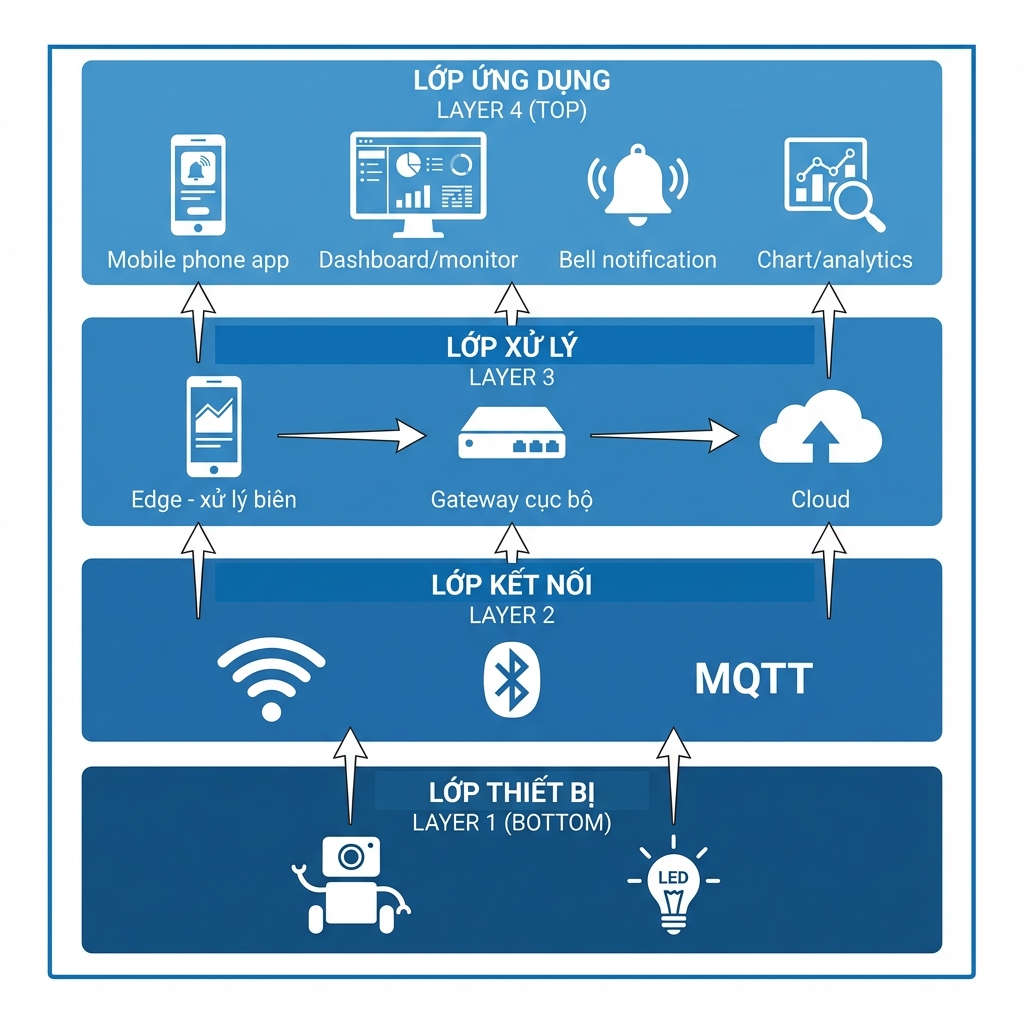
\includegraphics[width=0.85\textwidth]{Images/iot_architecture_layers.png}
%     \caption{Kiến trúc IoT 4 lớp cho hệ thống giám sát người cao tuổi}
%     \label{fig:iot_architecture}
% \end{figure}
% \newpage
% \textbf{a) Lớp Thiết bị (Device Layer)}

% Lớp thiết bị là tầng thấp nhất trong kiến trúc IoT, bao gồm các thiết bị vật lý trực tiếp tương tác với môi trường và người dùng:

% \begin{itemize}
%     \item \textbf{Robot}: Nền tảng OpenBot với khả năng di chuyển tự động, camera tích hợp để thu thập video stream, và các cảm biến khoảng cách để tránh vật cản. Robot đóng vai trò là ``mắt và tai'' di động của hệ thống, có thể tuần tra và tiếp cận người cao tuổi khi cần thiết.
    
%     \item \textbf{Actuators}: Các thiết bị chấp hành bao gồm đèn LED thông minh để cảnh báo bằng ánh sáng (nhấp nháy khi phát hiện té ngã), loa để phát thông báo bằng giọng nói (nhắc uống thuốc, cảnh báo nguy hiểm). Các actuator này được điều khiển qua giao thức MQTT, cho phép phản hồi nhanh trong các tình huống khẩn cấp.
% \end{itemize}

% \textbf{b) Lớp Kết nối (Connectivity Layer)}

% Lớp kết nối đảm bảo việc truyền dữ liệu giữa các thiết bị và hệ thống xử lý. Các giao thức được lựa chọn dựa trên yêu cầu về băng thông, độ trễ và tiêu thụ năng lượng:

% \begin{itemize}
%     \item \textbf{WiFi (IEEE 802.11)}: Giao thức kết nối chính cho smartphone (bộ não robot) và các thiết bị IoT với cloud. WiFi cung cấp băng thông cao (đủ cho video streaming) và được hỗ trợ rộng rãi trong môi trường gia đình. Smartphone kết nối qua WiFi để gửi video stream, nhận lệnh điều khiển, và đồng bộ dữ liệu với cloud.
    
%     \item \textbf{Bluetooth/BLE (Bluetooth Low Energy)}: Sử dụng cho kết nối tầm ngắn giữa smartphone và phần cứng robot (thay thế USB khi cần wireless), cũng như kết nối với các thiết bị đeo thông minh của người cao tuổi (vòng tay đo nhịp tim, nút bấm SOS). BLE tiêu thụ năng lượng thấp, phù hợp cho các thiết bị chạy pin.
    
%     \item \textbf{MQTT (Message Queuing Telemetry Transport)}: Giao thức nhắn tin publish-subscribe được thiết kế đặc biệt cho IoT. MQTT có header nhỏ (chỉ 2 bytes), phù hợp cho mạng có băng thông hạn chế và thiết bị tài nguyên thấp. Trong hệ thống, MQTT được sử dụng để:
%     \begin{itemize}
%         \item Gửi lệnh điều khiển từ ứng dụng người thân đến robot
%         \item Phát cảnh báo té ngã từ robot đến tất cả subscriber
%         \item Đồng bộ trạng thái thiết bị IoT (đèn, cửa, cảm biến)
%         \item Gửi heartbeat để giám sát trạng thái online của thiết bị
%     \end{itemize}
% \end{itemize}

% \textbf{c) Lớp Xử lý (Processing Layer)}

% Lớp xử lý đảm nhận việc phân tích dữ liệu và ra quyết định. Hệ thống áp dụng mô hình xử lý phân tán để tối ưu hóa độ trễ và chi phí:

% \begin{itemize}
%     \item \textbf{Edge Computing}: Xử lý trực tiếp trên smartphone (bộ não robot) với các tác vụ yêu cầu phản hồi real-time. Bao gồm:
%     \begin{itemize}
%         \item Chạy mô hình YOLOv11n để phát hiện té ngã với độ trễ $<$100ms
%         \item Xử lý ByteTrack để theo dõi người liên tục
%         \item Nhận diện giọng nói cục bộ (Vosk offline mode)
%         \item Điều khiển motor và phản hồi ngay lập tức
%     \end{itemize}
    
%     \item \textbf{Fog Computing}: Xử lý tại gateway cục bộ (có thể là router thông minh hoặc mini PC trong nhà) cho các tác vụ không yêu cầu phản hồi tức thì nhưng cần xử lý trước khi gửi lên cloud:
%     \begin{itemize}
%         \item Tổng hợp dữ liệu từ nhiều nguồn cảm biến
%         \item Cache video clips trước khi upload
%         \item Xử lý rule-based automation (bật đèn khi phát hiện chuyển động ban đêm)
%     \end{itemize}
    
%     \item \textbf{Cloud Computing}: Xử lý các tác vụ nặng và lưu trữ dài hạn trên cloud server:
%     \begin{itemize}
%         \item Chạy LLM API (GPT-4o, Gemini) cho chatbot thông minh
%         \item Lưu trữ lịch sử hoạt động và video clips
%         \item Huấn luyện và cập nhật mô hình AI
%         \item Phân tích pattern dài hạn để phát hiện bất thường
%     \end{itemize}
% \end{itemize}

% \textbf{d) Lớp Ứng dụng (Application Layer)}

% Lớp ứng dụng cung cấp giao diện người dùng và các tính năng cao cấp của hệ thống:

% \begin{itemize}
%     \item \textbf{Dashboard giám sát thời gian thực}: Giao diện web hiển thị trạng thái hệ thống, vị trí robot, video stream trực tiếp, và các cảnh báo. Dashboard cho phép người quản trị theo dõi nhiều thiết bị cùng lúc và can thiệp khi cần thiết.
    
%     \item \textbf{Ứng dụng mobile cho người chăm sóc}: Ứng dụng Android/iOS cho phép người thân:
%     \begin{itemize}
%         \item Nhận push notification khi phát hiện té ngã
%         \item Xem video stream từ robot theo thời gian thực
%         \item Điều khiển robot từ xa bằng virtual joystick
%         \item Thiết lập lịch nhắc uống thuốc và theo dõi tuân thủ
%         \item Thực hiện video call với người cao tuổi qua robot
%     \end{itemize}
    
%     \item \textbf{Hệ thống cảnh báo tự động}: Khi phát hiện sự cố (té ngã, bất động quá lâu, người lạ xâm nhập), hệ thống tự động:
%     \begin{itemize}
%         \item Phát cảnh báo âm thanh và ánh sáng tại chỗ
%         \item Gửi push notification đến tất cả người thân đã đăng ký
%         \item Lưu video clip trước và sau sự cố
%         \item Nếu không có phản hồi sau 2 phút, tự động gọi số khẩn cấp
%     \end{itemize}
    
%     \item \textbf{Phân tích dữ liệu và báo cáo}: Hệ thống tổng hợp dữ liệu hoạt động hàng ngày để:
%     \begin{itemize}
%         \item Tạo báo cáo tuân thủ uống thuốc (tuần/tháng)
%         \item Phân tích pattern hoạt động để phát hiện thay đổi bất thường
%         \item Thống kê thời gian hoạt động và nghỉ ngơi
%         \item Cung cấp insights cho bác sĩ hoặc người chăm sóc chuyên nghiệp
%     \end{itemize}
% \end{itemize}
% \subsubsection{Giao thức MQTT}

% MQTT (Message Queuing Telemetry Transport) là giao thức nhắn tin publish-subscribe được thiết kế cho IoT với các đặc điểm:

% \begin{itemize}
%     \item \textbf{Nhẹ}: Header tối thiểu 2 bytes, phù hợp thiết bị hạn chế tài nguyên
%     \item \textbf{Pub/Sub}: Mô hình publish-subscribe linh hoạt
%     \item \textbf{QoS}: Ba mức chất lượng dịch vụ (0, 1, 2)
%     \item \textbf{Retained Messages}: Lưu tin nhắn cuối cho subscriber mới
% \end{itemize}



\subsection{Giới thiệu YOLO (You Only Look Once)}
%=========================================

\subsubsection{Bài toán Object Detection}

Object Detection (Phát hiện đối tượng) là một trong những bài toán cơ bản và quan trọng nhất trong thị giác máy tính \reportcite{ref:odsurvey}. Khác với Image Classification chỉ xác định loại đối tượng chính trong ảnh, Object Detection yêu cầu đồng thời:

\begin{itemize}
    \item \textbf{Định vị (Localization)}: Xác định vị trí của đối tượng trong ảnh thông qua bounding box (hộp giới hạn)
    \item \textbf{Phân loại (Classification)}: Xác định loại của mỗi đối tượng được phát hiện
\end{itemize}

Trong bài toán phát hiện ngã, Object Detection đóng vai trò then chốt: mô hình cần xác định vị trí con người trong khung hình và phân loại trạng thái của họ (đang đứng, đi lại, hay đã ngã).

\subsubsection{Lịch sử phát triển Object Detection}

Theo khảo sát ``Object Detection in 20 Years'' của Zou và cộng sự \reportcite{ref:odsurvey}, lĩnh vực Object Detection đã trải qua sự phát triển đáng kể trong hơn hai thập kỷ:

\textbf{a) Giai đoạn truyền thống (1990s-2012)}

\begin{itemize}
    \item \textbf{Viola-Jones Detector (2001)}: Detector đầu tiên đạt tốc độ real-time cho face detection, sử dụng Haar-like features và AdaBoost
    \item \textbf{HOG Detector (2005)}: Histogram of Oriented Gradients cho pedestrian detection
    \item \textbf{DPM - Deformable Parts Model (2010)}: Mô hình biến dạng các phần, đạt SOTA trên PASCAL VOC nhiều năm
\end{itemize}

\textbf{b) Giai đoạn Deep Learning (2012-nay)}

\begin{itemize}
    \item \textbf{AlexNet (2012)}: Bước ngoặt của deep learning trong computer vision
    \item \textbf{R-CNN (2014)}: Kết hợp region proposals với CNN features
    \item \textbf{Fast R-CNN, Faster R-CNN (2015)}: Cải tiến tốc độ với RoI pooling và Region Proposal Network
    \item \textbf{YOLO v1 (2016)}: Đột phá với one-stage detection, real-time
    \item \textbf{SSD (2016)}: Single Shot MultiBox Detector với multi-scale features
    \item \textbf{RetinaNet (2017)}: Giới thiệu Focal Loss để giải quyết class imbalance
    \item \textbf{YOLO v3-v11 (2018-2024)}: Liên tục cải tiến về accuracy và speed
\end{itemize}

\textbf{c) Xu hướng hiện tại}

Theo \reportcite{ref:odsurvey}, các xu hướng chính trong Object Detection bao gồm:
\begin{itemize}
    \item Anchor-free detectors (loại bỏ anchor boxes)
    \item Transformer-based detectors (DETR, Swin Transformer)
    \item NAS-based architecture search (tự động tìm kiếm kiến trúc)
    \item Real-time detection trên edge devices
\end{itemize}

\subsubsection{Khái niệm Bounding Box}

Bounding Box (hộp giới hạn) là hình chữ nhật bao quanh đối tượng trong ảnh, được sử dụng để xác định vị trí và kích thước của đối tượng.

\begin{figure}[h!]
    \centering
    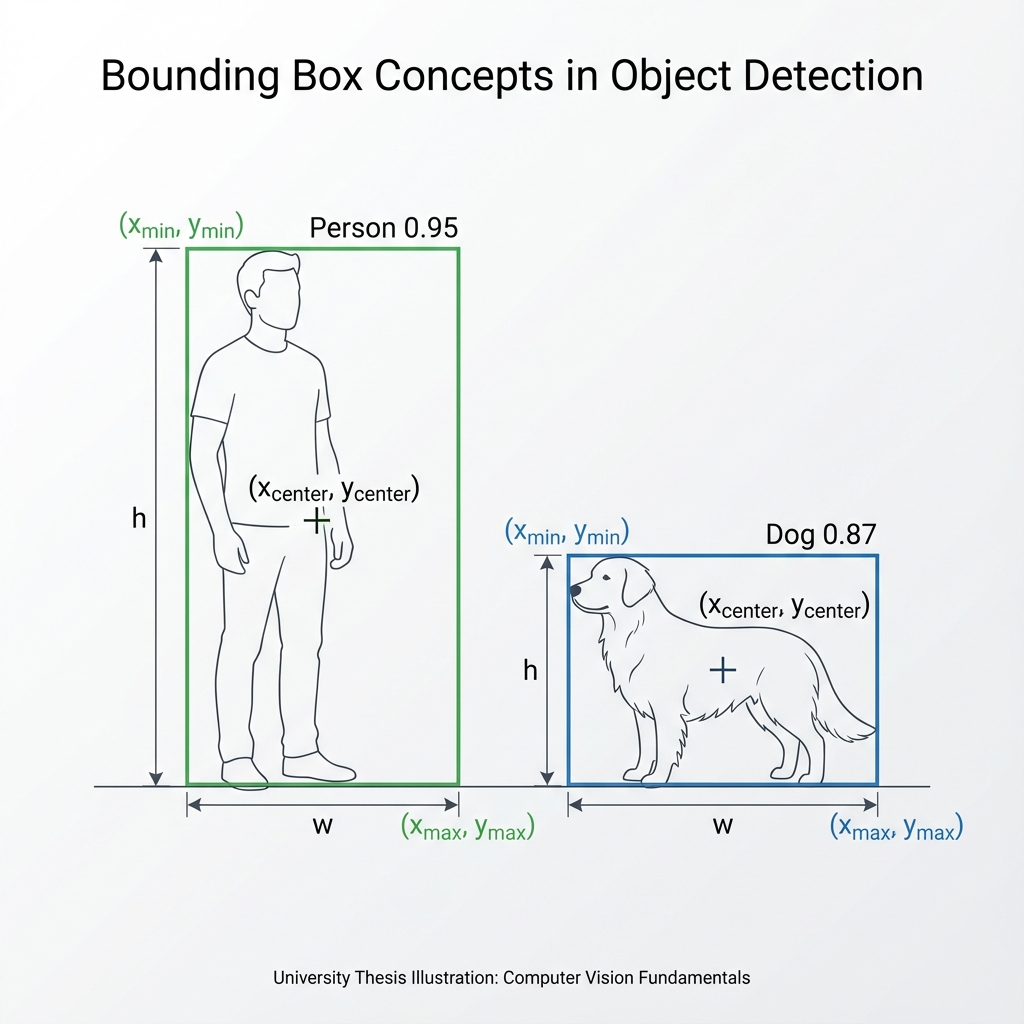
\includegraphics[width=0.6\textwidth]{Images/bounding_box_example.png}
    \vspace{8pt}
    \caption{Ví dụ minh họa Bounding Box trong Object Detection.}
    \label{fig:bounding_box}
\end{figure}

Có hai cách biểu diễn bounding box phổ biến:

\textbf{a) Format $(x_{min}, y_{min}, x_{max}, y_{max})$ - PASCAL VOC format}

\begin{itemize}
    \item $(x_{min}, y_{min})$: Tọa độ góc trên bên trái của box
    \item $(x_{max}, y_{max})$: Tọa độ góc dưới bên phải của box
    \item Đơn vị: pixel tuyệt đối
\end{itemize}

\textbf{b) Format $(x_{center}, y_{center}, w, h)$ - YOLO format}

\begin{itemize}
    \item $(x_{center}, y_{center})$: Tọa độ tâm của box
    \item $w$: Chiều rộng của box
    \item $h$: Chiều cao của box
    \item Đơn vị: normalized (chia cho kích thước ảnh, giá trị từ 0 đến 1)
\end{itemize}

\textbf{c) Công thức chuyển đổi}

Từ PASCAL VOC sang YOLO (với ảnh kích thước $W \times H$):
\begin{equation}
x_{center} = \frac{x_{min} + x_{max}}{2W}, \quad y_{center} = \frac{y_{min} + y_{max}}{2H}
\end{equation}
\begin{equation}
w = \frac{x_{max} - x_{min}}{W}, \quad h = \frac{y_{max} - y_{min}}{H}
\end{equation}

\subsubsection{Intersection over Union (IoU)}

IoU là metric đo độ chồng lấp giữa hai bounding box, được sử dụng rộng rãi trong đánh giá object detection:

\begin{equation}
IoU = \frac{\text{Area of Intersection}}{\text{Area of Union}} = \frac{|A \cap B|}{|A \cup B|}
\end{equation}

Trong đó:
\begin{itemize}
    \item $A$: Bounding box dự đoán (predicted)
    \item $B$: Bounding box ground truth (thực tế)
    \item IoU = 1: Hai box trùng khớp hoàn toàn
    \item IoU = 0: Hai box không có phần giao nhau
\end{itemize}

Ngưỡng IoU thường được sử dụng để xác định dự đoán đúng:
\begin{itemize}
    \item IoU $\geq 0.5$: Ngưỡng phổ biến (PASCAL VOC, COCO mAP@0.5)
    \item IoU $\geq 0.75$: Ngưỡng nghiêm ngặt (COCO mAP@0.75)
    \item IoU từ 0.5 đến 0.95: Đánh giá đa ngưỡng (COCO mAP@[.5:.95])
\end{itemize}

\subsubsection{Các khái niệm True Positive, False Positive, False Negative}

Để đánh giá kết quả detection, cần phân loại các dự đoán:

\begin{itemize}
    \item \textbf{True Positive (TP)}: Dự đoán đúng - có bounding box dự đoán khớp với ground truth (IoU $\geq$ threshold) và đúng class
    \item \textbf{False Positive (FP)}: Dự đoán sai - bounding box dự đoán không khớp với bất kỳ ground truth nào, hoặc sai class
    \item \textbf{False Negative (FN)}: Bỏ sót - ground truth không được detect bởi bất kỳ dự đoán nào
\end{itemize}

Từ đó tính được:
\begin{equation}
\text{Precision} = \frac{TP}{TP + FP} = \frac{\text{Số dự đoán đúng}}{\text{Tổng số dự đoán}}
\end{equation}
\begin{equation}
\text{Recall} = \frac{TP}{TP + FN} = \frac{\text{Số dự đoán đúng}}{\text{Tổng số ground truth}}
\end{equation}

\subsubsection{Đánh giá hiệu suất: Mean Average Precision (mAP)}

Mean Average Precision (mAP) là metric chuẩn để đánh giá hiệu suất của mô hình object detection, tổng hợp cả precision và recall.

\textbf{a) Precision-Recall Curve}

Với mỗi class, sắp xếp các dự đoán theo confidence score giảm dần. Tại mỗi điểm, tính precision và recall tích lũy, từ đó vẽ được đường cong Precision-Recall.

\textbf{b) Average Precision (AP)}

AP là diện tích dưới đường cong Precision-Recall:
\begin{equation}
AP = \int_0^1 p(r) \, dr
\end{equation}

Trong thực tế, sử dụng phép nội suy (interpolation):
\begin{equation}
AP = \sum_{i=1}^{n} (r_i - r_{i-1}) \cdot p_{interp}(r_i)
\end{equation}

với $p_{interp}(r) = \max_{r' \geq r} p(r')$ là precision nội suy tại recall $r$.

\textbf{c) Mean Average Precision (mAP)}

mAP là trung bình của AP trên tất cả các class:
\begin{equation}
mAP = \frac{1}{N} \sum_{i=1}^{N} AP_i
\end{equation}

với $N$ là số class trong dataset.

\textbf{d) Các biến thể mAP}

\begin{itemize}
    \item \textbf{mAP@0.5 (mAP50)}: AP tính với ngưỡng IoU = 0.5, được sử dụng trong PASCAL VOC
    \item \textbf{mAP@0.75 (mAP75)}: AP với ngưỡng IoU = 0.75, nghiêm ngặt hơn
    \item \textbf{mAP@[.5:.95]}: Trung bình AP với IoU từ 0.5 đến 0.95 (bước 0.05), metric chính của COCO
    \item \textbf{mAP Small/Medium/Large}: mAP theo kích thước đối tượng
\end{itemize}

\textbf{e) Ý nghĩa của mAP}

\begin{itemize}
    \item mAP cao $\rightarrow$ Mô hình phát hiện đúng nhiều đối tượng và định vị chính xác
    \item mAP50 cao nhưng mAP75 thấp $\rightarrow$ Phát hiện được nhưng định vị chưa chính xác
    \item Precision cao, Recall thấp $\rightarrow$ Mô hình thận trọng, ít false positive nhưng bỏ sót nhiều
    \item Precision thấp, Recall cao $\rightarrow$ Mô hình phát hiện nhiều nhưng có nhiều false positive
\end{itemize}

\subsubsection{Ý tưởng YOLO: Phát hiện trong một lần suy luận}

YOLO (You Only Look Once) được Joseph Redmon, Santosh Divvala, Ross Girshick và Ali Farhadi đề xuất năm 2016 trong bài báo ``You Only Look Once: Unified, Real-Time Object Detection'' \reportcite{ref:yolo}. Đây là bước đột phá mang đến cách tiếp cận hợp nhất cho Object Detection.

\textbf{Ý tưởng cốt lõi của YOLO} (theo \reportcite{ref:yolo}):

``We reframe object detection as a single regression problem, straight from image pixels to bounding box coordinates and class probabilities. Using our system, you only look once (YOLO) at an image to predict what objects are present and where they are.''

Thay vì coi detection như bài toán phân loại (classifier), YOLO đặt lại vấn đề như bài toán hồi quy về tọa độ bounding box và xác suất class, tất cả trong một lần forward pass duy nhất qua mạng neural.

\textbf{Nguyên lý hoạt động của YOLO:}

\begin{enumerate}
    \item \textbf{Chia lưới}: Ảnh đầu vào được chia thành lưới $S \times S$ ô (grid cells). Trong paper gốc, $S = 7$.

    \begin{figure}[h!]
        \centering
        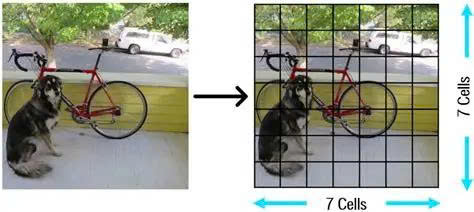
\includegraphics[width=0.7\textwidth]{Images/7x7.jpg}
        \vspace{8pt}
        \caption{Minh họa chia lưới $7 \times 7$ trong YOLO: mỗi ô chịu trách nhiệm phát hiện đối tượng có tâm nằm trong ô đó.}
        \label{fig:yolo_grid}
    \end{figure}
    \item \textbf{Dự đoán bounding boxes}: Mỗi ô dự đoán $B$ bounding boxes (mặc định $B = 2$) cùng với điểm confidence.
    \item \textbf{Dự đoán class probabilities}: Mỗi ô dự đoán $C$ xác suất class có điều kiện $Pr(Class_i|Object)$.
    \item \textbf{Tensor đầu ra}: Kích thước $S \times S \times (B \times 5 + C)$. Với PASCAL VOC ($C=20$), tensor có kích thước $7 \times 7 \times 30$.
    \item \textbf{Post-processing}: Non-Maximum Suppression (NMS) loại bỏ các box trùng lặp.
\end{enumerate}

\textbf{Đầu ra của mỗi bounding box bao gồm 5 giá trị:}
\begin{itemize}
    \item $(x, y)$: Tọa độ tâm của box tương đối với ô lưới (normalized 0-1 trong ô)
    \item $(w, h)$: Chiều rộng và chiều cao của box tương đối với toàn ảnh (normalized 0-1)
    \item $confidence = Pr(Object) \times IOU^{truth}_{pred}$: Độ tin cậy rằng box chứa đối tượng VÀ độ chính xác của box so với ground truth
\end{itemize}

\textbf{Hiệu suất của YOLO theo bài báo gốc:}
\begin{itemize}
    \item Base YOLO: 45 FPS (frames per second) trên GPU
    \item Fast YOLO: 155 FPS - nhanh hơn gấp đôi các detector real-time khác
    \item mAP trên PASCAL VOC 2007: 63.4\% (base), 52.7\% (fast)
\end{itemize}

\subsubsection{So sánh YOLO với phương pháp truyền thống}

\begin{table}[h]
\centering
\caption{So sánh YOLO với các phương pháp Object Detection khác}
\begin{tabular}{|l|c|c|c|}
\hline
\textbf{Phương pháp} & \textbf{Tốc độ (FPS)} & \textbf{mAP} & \textbf{Thời gian thực} \\
\hline
R-CNN & 0.02 & 53.7 & Không \\
Fast R-CNN & 0.5 & 70.0 & Không \\
Faster R-CNN & 7-17 & 73.2 & Khó \\
YOLO v1 & 45 & 63.4 & Có \\
YOLOv3 & 30-50 & 57.9 & Có \\
YOLOv5 & 100+ & 68.9 & Có \\
\hline
\end{tabular}
\end{table}

\textbf{Ưu điểm của YOLO:}
\begin{itemize}
    \item Tốc độ: Xử lý real-time với hàng chục đến hàng trăm FPS
    \item Đơn giản: Một mạng duy nhất, dễ huấn luyện end-to-end
    \item Nhìn toàn cục: Xem xét toàn bộ ảnh khi dự đoán, hiểu được ngữ cảnh tốt hơn
    \item Tổng quát hóa tốt: Ít false positive trên background so với các phương pháp dựa trên sliding window
\end{itemize}

\textbf{Hạn chế:}
\begin{itemize}
    \item Khó phát hiện các đối tượng nhỏ hoặc xếp chồng nhau
    \item Độ chính xác định vị có thể kém hơn phương pháp hai giai đoạn ở một số trường hợp
\end{itemize}

%=========================================
\subsection{Nền tảng Thị giác máy tính (Computer Vision)}

Thị giác máy tính (Computer Vision) đóng vai trò cốt lõi trong hệ thống giám sát và nhận diện té ngã. Bằng cách phân tích luồng video từ camera, hệ thống có khả năng nhận biết, định vị và theo dõi con người trong không gian. Phần này trình bày các nền tảng kỹ thuật được sử dụng bao gồm Mạng nơ-ron tích chập (CNN), kiến trúc YOLO cho bài toán phát hiện đối tượng và thuật toán ByteTrack cho bài toán theo dõi.

\subsubsection{Mạng nơ-ron tích chập (CNN) và Kiến trúc YOLO26}

\textbf{Mạng nơ-ron tích chập (CNN)}

Mạng nơ-ron tích chập (Convolutional Neural Network - CNN) là một lớp mạng học sâu (Deep Learning) chuyên biệt, được thiết kế để xử lý dữ liệu có dạng lưới tĩnh như hình ảnh 2D
\reportcite{ref:cnn}. Khác với mạng đa tầng (MLP) truyền thống yêu cầu làm phẳng (flatten) hình ảnh gây mất thông tin không gian, CNN bảo toàn cấu trúc không gian của pixel bằng cách sử dụng các bộ lọc (filters/kernels) trượt qua toàn bộ bức ảnh.

Kiến trúc cốt lõi của một mạng CNN tiêu chuẩn bao gồm 3 loại lớp chính:
\begin{itemize}
    \item \textbf{Lớp tích chập (Convolutional Layer)}: Đóng vai trò là bộ trích xuất đặc trưng (feature extractor). Nó áp dụng các phép tính tích chập giữa một bộ lọc ma trận (kernel) và vùng ảnh đầu vào để tạo ra các bản đồ đặc trưng (feature maps). Ở các lớp đầu, CNN học cách nhận diện các đặc trưng cấp thấp như cạnh, góc; ở các lớp sâu hơn, nó nhận diện các đặc trưng phức tạp như hình khối, khuôn mặt.
    \item \textbf{Lớp gộp (Pooling Layer)}: Thường theo ngay sau lớp tích chập (như Max Pooling hoặc Average Pooling), có nhiệm vụ giảm độ phân giải không gian của bản đồ đặc trưng. Quá trình này không chỉ giúp giảm đáng kể khối lượng tính toán, tránh hiện tượng quá khớp (overfitting) mà còn mang lại tính bất biến cục bộ (translation invariance) -- giúp mô hình vẫn nhận diện được đối tượng dù chúng bị dịch chuyển nhẹ trong khung hình.
    \item \textbf{Lớp kết nối đầy đủ (Fully Connected Layer)}: Nằm ở phần cuối mạng, làm nhiệm vụ tổng hợp các đặc trưng cao cấp đã được trích xuất để thực hiện dự đoán cuối cùng (phân loại hoặc hồi quy tọa độ).
\end{itemize}

Bên cạnh đó, sau mỗi lớp tích chập, một hàm kích hoạt phi tuyến (như ReLU, SiLU) được áp dụng để đưa tính phi tuyến vào mô hình, cho phép CNN học được các mối quan hệ phức tạp. Sự kết hợp luân phiên giữa Convolution và Pooling giúp CNN tự động học cách phân tích hình ảnh mà không cần đến các chuyên gia thiết kế đặc trưng thủ công (manual feature engineering) như các phương pháp thị giác máy tính cổ điển.

\begin{figure}[htbp]
    \centering
    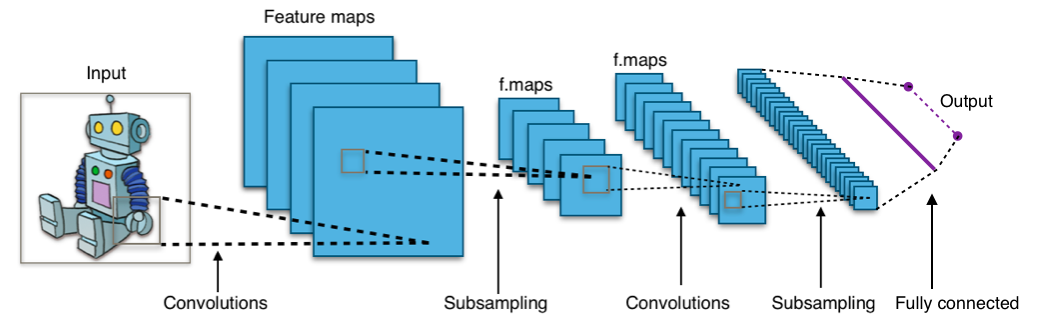
\includegraphics[width=0.9\textwidth]{Images/cnn_arch.png}
    \caption{Minh họa cấu trúc tiêu biểu của mạng nơ-ron tích chập (CNN) gồm các lớp Convolution, Pooling và Fully Connected.}
    \label{fig:typical_cnn}
\end{figure}

\textbf{Kiến trúc YOLO26 (Kế thừa từ YOLOv8/YOLOv11)}
YOLO (You Only Look Once) là một trong những họ mô hình Object Detection tốc độ cao phổ biến nhất. Khác với các phương pháp dựa trên region-proposal (như Faster R-CNN) yêu cầu chạy mô hình nhiều lần trên một ảnh, YOLO định hình bài toán detection như một bài toán hồi quy đơn lẻ (single regression problem) dự đoán trực tiếp tọa độ Bounding Box và xác suất nhãn lớp từ các pixel hình ảnh trong một lần quét duy nhất
\reportcite{ref:yolo}.

Trong hệ thống, mô hình YOLO26 (phiên bản nano tối ưu từ YOLO-Pose) được sử dụng nhằm mục đích trích xuất khung xương (pose landmarks) thay vì chỉ lấy bounding box thông thường.
Mô hình này nổi bật với các cải tiến kiến trúc như:
\begin{itemize}
    \item \textbf{Backbone hiệu năng cao}: Sử dụng các khối C3k2 (Cross Stage Partial) giúp giảm tham số nhưng vẫn duy trì độ chính xác cao.
    \item \textbf{Đầu ra đa nhiệm (Multi-task Head)}: Hỗ trợ dự đoán đồng thời vị trí Bounding Box và 17 điểm khớp xương (keypoints) của con người.
    \item \textbf{Tối ưu hóa cho thiết bị biên (Edge Devices)}: Phiên bản nano (yolo26n-pose) có dung lượng cực nhẹ, phù hợp để chuyển đổi sang định dạng TFLite hoặc ONNX, giúp hệ thống đạt tốc độ Real-time trên các phần cứng hạn chế như Raspberry Pi hay điện thoại di động.
\end{itemize}

\begin{figure}[htbp]
    \centering
    
\includegraphics[width=0.8\textwidth]{yolo_arch.jpg}
    \caption{Minh họa một kiến trúc mạng YOLO tiêu biểu với Backbone, Neck và Head.}
    \label{fig:yolo_architecture}
\end{figure}

\subsubsection{Thuật toán theo dõi đa đối tượng ByteTrack}

Trong bài toán nhận diện té ngã, không chỉ cần phát hiện người ở từng khung hình (frame) riêng lẻ, mà còn phải liên kết các phát hiện đó xuyên suốt thời gian để tạo thành một chuỗi hành động (tracklet). Đây là vai trò của bài toán Theo dõi đa đối tượng (Multi-Object Tracking - MOT).

Hệ thống ứng dụng thuật toán \textbf{ByteTrack}, một trong những thuật toán tracking State-of-the-Art hiện nay với phương pháp tiếp cận độc đáo về ghép nối dữ liệu (data association)
\reportcite{ref:bytetrack}.

\textbf{Cơ chế hoạt động của ByteTrack:}
Các thuật toán tracking truyền thống thường loại bỏ hoàn toàn các detection có độ tin cậy thấp (low-confidence) nhằm giảm thiểu nhiễu. Tuy nhiên, điều này dẫn đến việc mất dấu đối tượng khi họ bị che khuất một phần (occlusion) hoặc hình ảnh bị mờ do chuyển động nhanh (thường gặp khi nạn nhân đang ngã).

ByteTrack giải quyết vấn đề này bằng kỹ thuật \textbf{Dual-threshold Association} (Liên kết hai ngưỡng):
\begin{enumerate}
    \item \textbf{Ghép nối lần 1 (High-score association)}: Thuật toán sử dụng bộ lọc Kalman (Kalman Filter) để dự đoán vị trí của đối tượng ở frame tiếp theo. Sau đó, nó tính toán khoảng cách IoU (Intersection over Union) giữa vị trí dự đoán và các bounding box có độ tin cậy \textit{cao} do YOLO trả về. Các cặp phù hợp sẽ được liên kết với nhau.
    \item \textbf{Ghép nối lần 2 (Low-score association)}: Đối với các đối tượng chưa tìm được ghép nối (unmatched tracks) ở lần 1, ByteTrack không xóa chúng đi mà tiếp tục tìm kiếm trong nhóm các bounding box có độ tin cậy \textit{thấp}. Nếu nạn nhân đang ngã bị mờ, YOLO có thể trả về box với độ tin cậy thấp. Nhờ bước thứ hai này, ByteTrack có thể "cứu" lại tracklet của nạn nhân, giúp chuỗi hành động không bị ngắt quãng.
\end{enumerate}

\begin{figure}[htbp]
    \centering
    
\includegraphics[width=0.9\textwidth]{bytetrack_arch.jpg}
    \caption{Thuật toán ByteTrack với cơ chế Dual-threshold Association giúp duy trì Track ID ổn định.}
    \label{fig:bytetrack}
\end{figure}

Sự kết hợp giữa YOLO26 (nhận diện chính xác, nhanh) và ByteTrack (liên kết mạnh mẽ, chống đứt gãy) tạo nên một nền tảng vững chắc để trích xuất dữ liệu chuỗi thời gian chất lượng cao, trước khi đưa vào mạng LSTM phân tích hành vi ngã.




% --- Tích hợp từ phần cũ ---

Tracking-by-detection tách bài toán thành phát hiện đối tượng ở mỗi frame và liên kết detection qua thời gian. SORT sử dụng Kalman để dự báo chuyển động, IoU làm độ tương đồng và Hungarian cho phép gán tối ưu \reportcite{ref:sort}. Deep SORT bổ sung embedding ngoại hình để giảm đổi ID khi che khuất \reportcite{ref:deepsort}; ByteTrack chỉ ra rằng các detection confidence thấp vẫn có thể hữu ích khi liên kết với track \reportcite{ref:bytetrack}.

Kalman gồm hai pha. Pha dự báo:

\begin{align}
\hat{x}_{t|t-1}&=F\hat{x}_{t-1|t-1}+Bu_t,\\
P_{t|t-1}&=FP_{t-1|t-1}F^T+Q.
\end{align}

Pha cập nhật với quan sát $z_t$:

\begin{align}
K_t&=P_{t|t-1}H^T(HP_{t|t-1}H^T+R)^{-1},\\
\hat{x}_{t|t}&=\hat{x}_{t|t-1}+K_t(z_t-H\hat{x}_{t|t-1}),\\
P_{t|t}&=(I-K_tH)P_{t|t-1}.
\end{align}

Ma trận chi phí giữa $n$ track và $m$ detection được đưa vào thuật toán Hungarian, vốn giải bài toán gán tuyến tính \reportcite{ref:hungarian}. IoU đơn độc có thể thất bại khi người từ đứng chuyển sang nằm làm vùng bao thay đổi mạnh. Vì vậy đề tài kết hợp IoU, khoảng cách tâm, neo vai/hông, tỷ lệ diện tích và histogram vùng thân. Định danh ID0 còn được bảo vệ bởi tuổi track dài hơn và phục hồi có điều kiện.


\subsection{Mô hình chuỗi thời gian (Sequence Modeling)}
%=========================================

\subsubsection{Mạng nơ-ron hồi quy (RNN)}

Mạng nơ-ron hồi quy (Recurrent Neural Network - RNN) là một lớp mạng nơ-ron nhân tạo chuyên biệt để xử lý dữ liệu dạng chuỗi (sequence data) như văn bản, âm thanh, hoặc chuỗi thời gian (time-series). Trong ngữ cảnh phát hiện té ngã, luồng video chứa các khung hình liên tiếp tạo thành một chuỗi dữ liệu thời gian ghi nhận chuyển động của con người
\reportcite{ref:rnn}.

Khác với mạng truyền thẳng (Feedforward Neural Network) nơi dữ liệu chỉ đi một chiều từ đầu vào đến đầu ra, RNN sở hữu các "vòng lặp" (loops) cho phép thông tin có thể lưu lại và truyền qua các bước thời gian.
Nhờ cơ chế trạng thái ẩn (hidden state), mạng RNN có thể nhớ được thông tin từ quá khứ để ảnh hưởng đến quyết định ở hiện tại. Tuy nhiên, RNN truyền thống gặp phải vấn đề \textbf{triệt tiêu đạo hàm (vanishing gradient)} và \textbf{bùng nổ đạo hàm (exploding gradient)} khi phải học các phụ thuộc xa (long-term dependencies) trong những chuỗi dữ liệu dài.

\subsubsection{Mạng Bộ nhớ Ngắn-Dài hạn (LSTM)}

Để khắc phục nhược điểm của RNN, mạng \textbf{Long Short-Term Memory (LSTM)} được đề xuất bởi Hochreiter và Schmidhuber (1997)
\reportcite{ref:lstm}. LSTM có khả năng học các phụ thuộc dài hạn cực kỳ xuất sắc nhờ cấu trúc "Cell State" (trạng thái tế bào) hoạt động như một băng chuyền thông tin xuyên suốt các bước thời gian, giúp đạo hàm không bị suy giảm quá nhanh.

Cốt lõi của kiến trúc LSTM nằm ở ba cổng (gates) đóng vai trò kiểm soát luồng thông tin:
\begin{itemize}
    \item \textbf{Cổng quên (Forget Gate)}: Quyết định lượng thông tin từ quá khứ (trạng thái tế bào trước đó) cần bị loại bỏ hoặc lãng quên.
    \item \textbf{Cổng đầu vào (Input Gate)}: Quyết định lượng thông tin mới (từ dữ liệu hiện tại và trạng thái ẩn trước đó) nào sẽ được cập nhật vào trạng thái tế bào.
    \item \textbf{Cổng đầu ra (Output Gate)}: Quyết định thông tin nào từ trạng thái tế bào sẽ được xuất ra dưới dạng trạng thái ẩn mới cho bước thời gian tiếp theo.
\end{itemize}

\begin{figure}[htbp]
    \centering
    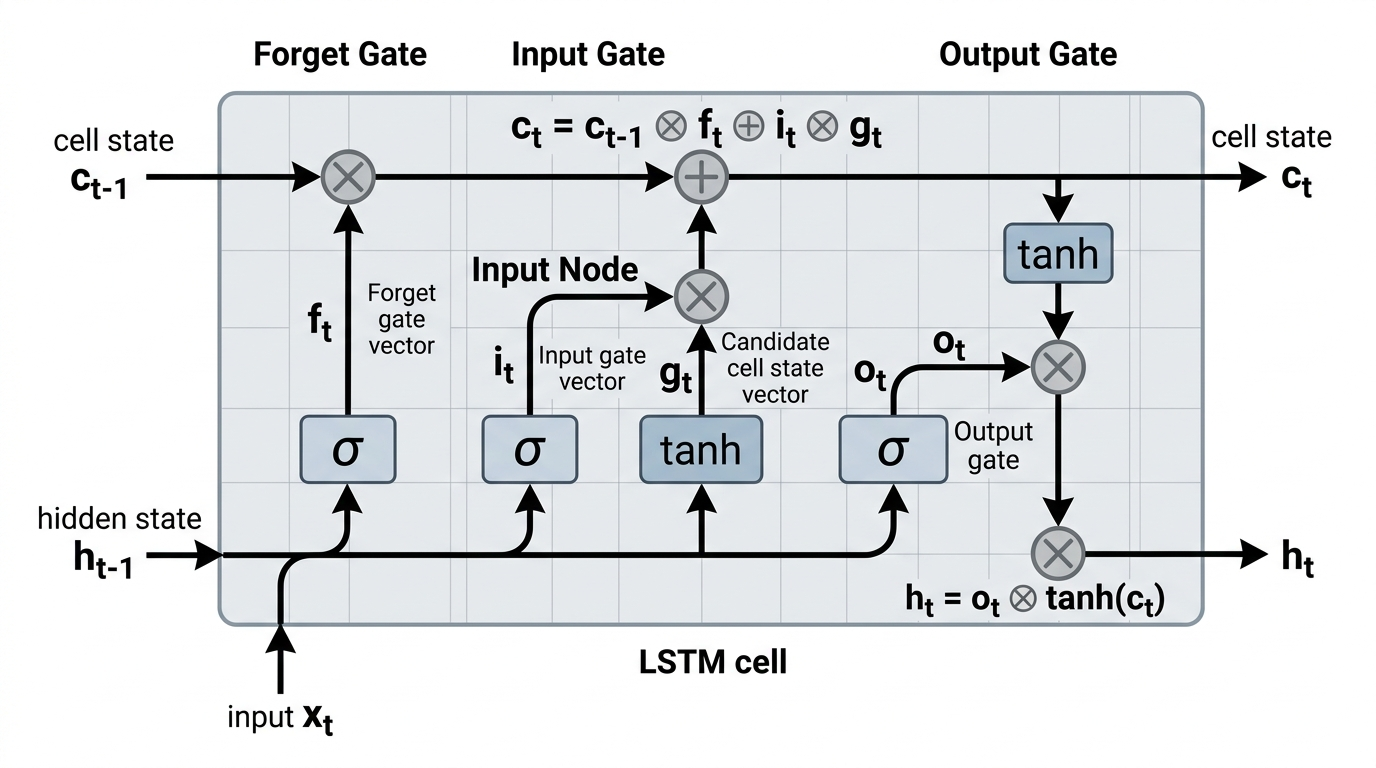
\includegraphics[width=0.9\textwidth]{Images/lstm_arch.jpg}
    \caption{Cấu trúc chi tiết của một tế bào LSTM (LSTM cell) với hệ thống các cổng kiểm soát thông tin.}
    \label{fig:lstm_architecture}
\end{figure}

Trong kiến trúc của hệ thống nhận diện té ngã, LSTM đóng vai trò cực kỳ quan trọng ở khâu cuối cùng. Sau khi mạng YOLO và thuật toán ByteTrack trích xuất ra một chuỗi các tọa độ điểm neo (keypoints) xuyên suốt các khung hình, dữ liệu này mang tính chất chuỗi thời gian. Mạng LSTM sẽ tiếp nhận chuỗi tọa độ này, phân tích sự thay đổi vị trí không gian của cơ thể con người theo thời gian, từ đó nhận diện được hành động ngã một cách chính xác so với các hành động bình thường như ngồi, cúi người hay nằm.



% --- Tích hợp từ phần cũ ---

Một detector trên từng ảnh chỉ quan sát tư thế tại một thời điểm. Trong bài toán té ngã, quá trình chuyển từ đứng/ngồi sang hạ thấp nhanh rồi nằm mới là tín hiệu quan trọng. Recurrent Neural Network (RNN) đưa trạng thái ẩn từ bước $t-1$ sang bước $t$, nhưng có thể gặp mất hoặc bùng nổ gradient khi chuỗi dài. Long Short-Term Memory (LSTM) bổ sung cell state và ba cổng vào, quên, ra để điều tiết thông tin \reportcite{ref:lstm}.

Với input $x_t$, hidden state $h_{t-1}$ và cell state $c_{t-1}$:

\begin{align}
f_t &= \sigma(W_f[x_t,h_{t-1}]+b_f),\\
i_t &= \sigma(W_i[x_t,h_{t-1}]+b_i),\\
\tilde{c}_t &= \tanh(W_c[x_t,h_{t-1}]+b_c),\\
c_t &= f_t\odot c_{t-1}+i_t\odot\tilde{c}_t,\\
o_t &= \sigma(W_o[x_t,h_{t-1}]+b_o),\\
h_t &= o_t\odot\tanh(c_t).
\end{align}

Trong hệ thống, một mẫu là tensor $X\in\mathbb{R}^{15\times69}$. Số 15 là chiều thời gian; 69 là vector pose/hình học mỗi frame. Đầu ra softmax hai lớp được diễn giải là normal/fall. Threshold xác suất chỉ là tầng đầu; hysteresis theo số frame liên tiếp và hậu kiểm hình học giúp ngăn trạng thái dao động. Cần lưu ý nếu FPS thay đổi, 15 frame tương ứng thời gian thực khác nhau; một triển khai tốt nên log timestamp hoặc resample chuỗi theo thời gian.


\subsection{Xử lý Ngôn ngữ Tự nhiên (NLP) và Hệ thống Giọng nói}
%=========================================

\subsubsection{Mô hình ngôn ngữ lớn (LLM) và Kiến trúc Transformer}

Mô hình ngôn ngữ lớn (Large Language Model - LLM) là một bước đột phá trong lĩnh vực Trí tuệ Nhân tạo, được huấn luyện trên lượng dữ liệu văn bản khổng lồ để có khả năng hiểu, suy luận và tạo ra ngôn ngữ tự nhiên giống con người. Trái tim của các mô hình LLM hiện đại chính là kiến trúc \textbf{Transformer} \reportcite{ref:transformer}.

Kiến trúc Transformer loại bỏ hoàn toàn cơ chế xử lý tuần tự của RNN/LSTM, thay vào đó sử dụng cơ chế \textbf{Tự chú ý (Self-Attention)}. Cơ chế này cho phép mô hình đánh giá mức độ liên quan (trọng số) của từng từ trong câu với tất cả các từ khác cùng một lúc, bất kể khoảng cách giữa chúng. Nhờ đó, Transformer không chỉ giải quyết triệt để vấn đề quên thông tin tầm xa mà còn hỗ trợ tính toán song song, giúp tăng tốc độ huấn luyện lên nhiều lần.

\begin{figure}[htbp]
    \centering
    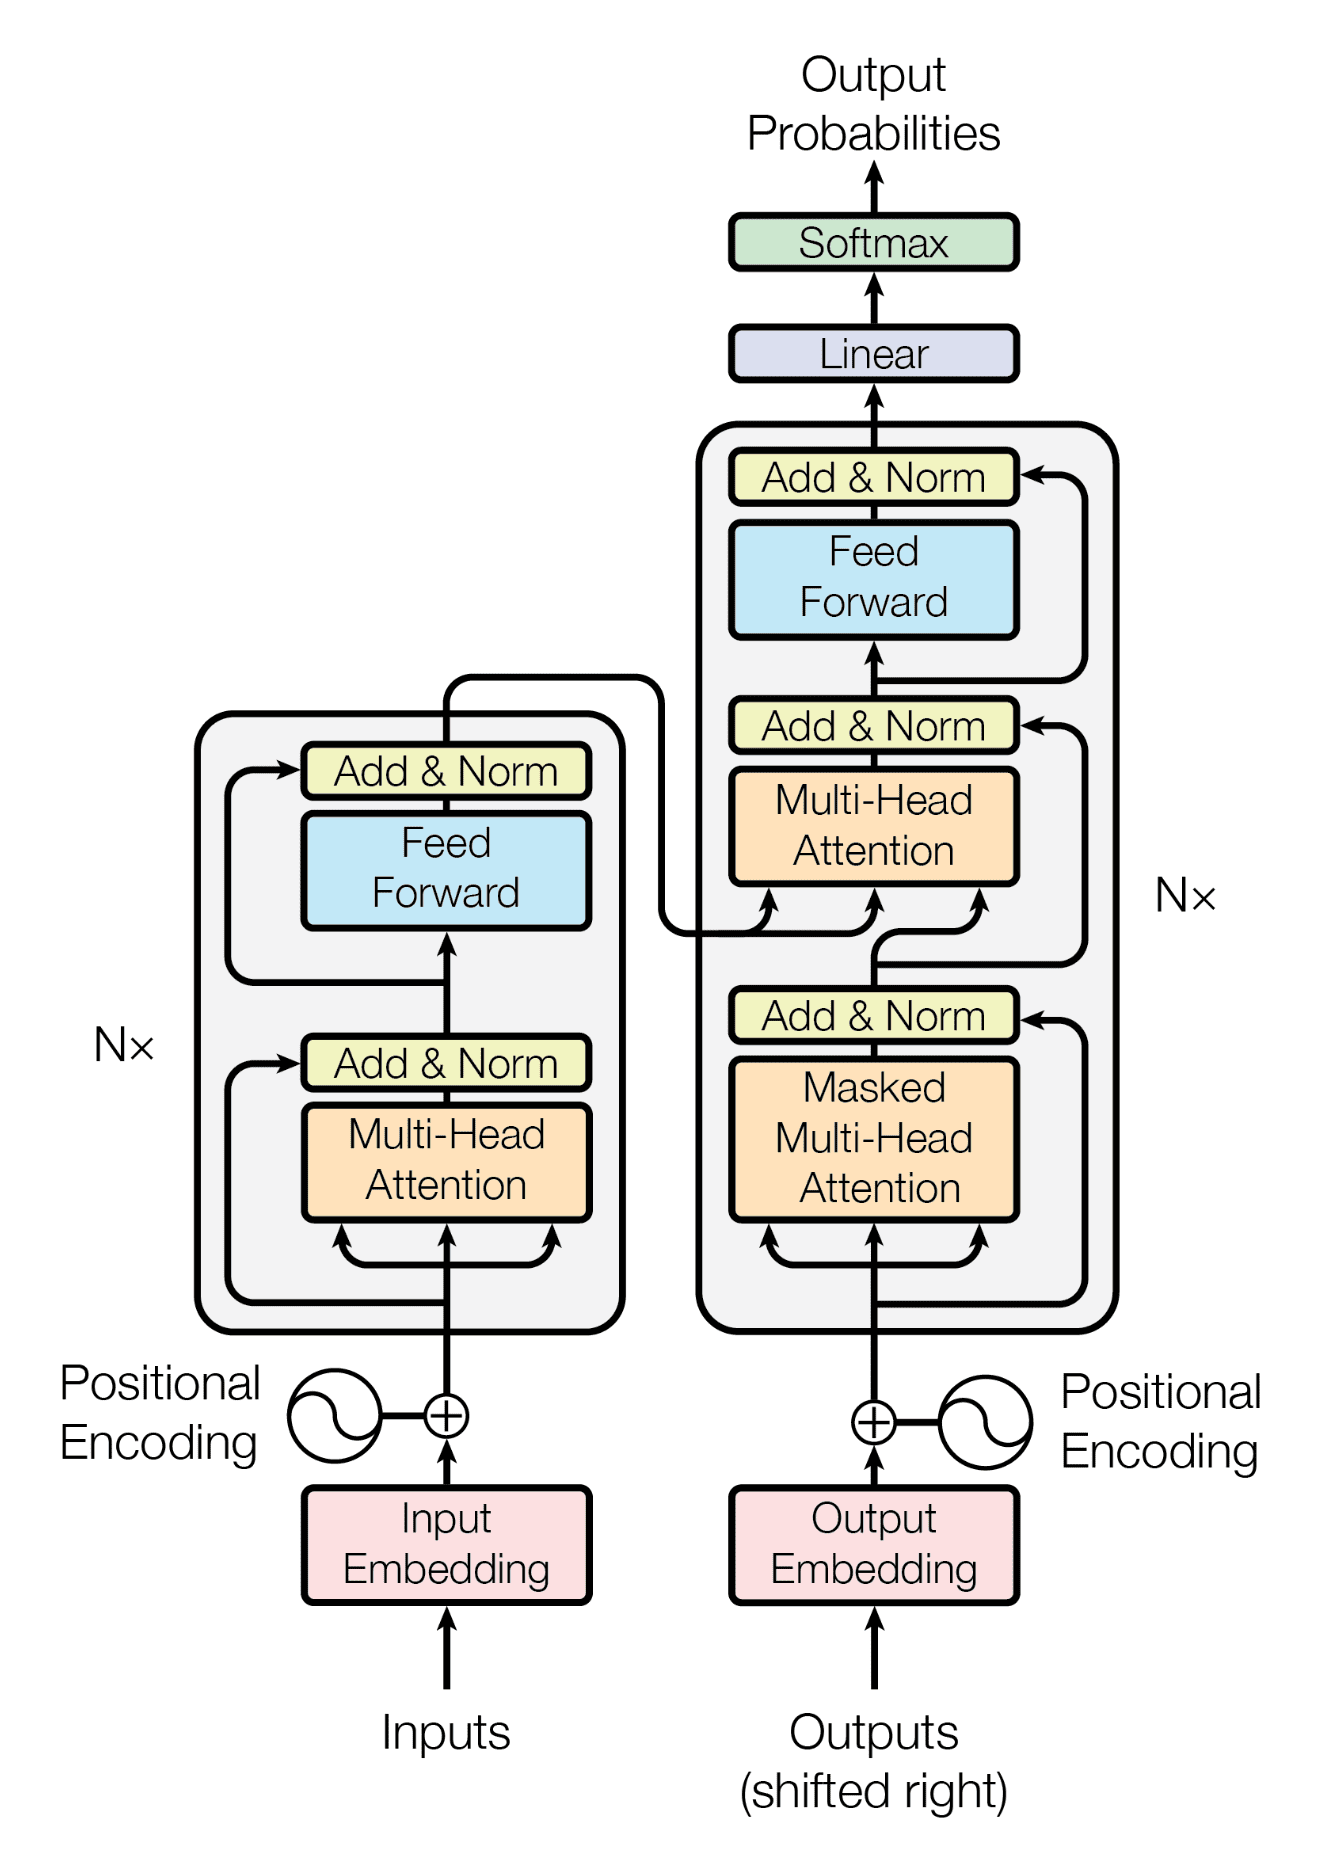
\includegraphics[width=0.6\textwidth]{Images/transformer_arch.png}
    \caption{Sơ đồ kiến trúc của mô hình Transformer với cơ chế Multi-Head Attention.}
    \label{fig:transformer}
\end{figure}

Trong phạm vi hệ thống robot hỗ trợ người cao tuổi, việc triển khai một mô hình LLM với hàng tỷ tham số trực tiếp trên phần cứng cục bộ (edge devices) là không khả thi do giới hạn về bộ nhớ và năng lượng. Do đó, hệ thống sử dụng \textbf{Groq API} để gọi các mô hình LLM mã nguồn mở (như LLaMA 3 hoặc Mixtral) thông qua điện toán đám mây \reportcite{ref:groq_api}. Điểm khác biệt của Groq là việc sử dụng chip LPU (Language Processing Unit) chuyên biệt cho inference, mang lại tốc độ phản hồi cực kỳ nhanh (có thể lên tới hàng trăm token/giây). Điều này rất quan trọng để đảm bảo robot có thể giao tiếp, nhắc nhở hoặc trò chuyện với người cao tuổi theo thời gian thực mà không có độ trễ gây khó chịu.


% --- Tích hợp từ phần cũ ---
%=========================================

\subsubsection{Khái niệm AI Agent}

AI Agent (Tác tử trí tuệ nhân tạo) là một hệ thống tự động có khả năng nhận thức môi trường, đưa ra quyết định, và thực hiện hành động để đạt được mục tiêu cụ thể. Khác với các chương trình truyền thống hoạt động theo luật cố định, AI Agent có khả năng:

\begin{itemize}
    \item \textbf{Tự chủ (Autonomy)}: Hoạt động độc lập mà không cần sự can thiệp liên tục của con người
    \item \textbf{Phản ứng (Reactivity)}: Nhận thức và phản hồi kịp thời với thay đổi của môi trường
    \item \textbf{Chủ động (Proactivity)}: Khởi xướng hành động để đạt mục tiêu, không chỉ phản ứng thụ động
    \item \textbf{Xã hội (Social ability)}: Tương tác và giao tiếp với con người hoặc các agent khác
\end{itemize}

Trong hệ thống robot giám sát người cao tuổi, AI Agent đóng vai trò là ``bộ não'' thông minh, điều phối các thành phần khác nhau (camera, cảm biến, IoT) và giao tiếp tự nhiên với người dùng.

\subsubsection{Mô hình Ngôn ngữ Lớn (Large Language Models)}

Large Language Models (LLM) là các mô hình học sâu được huấn luyện trên lượng dữ liệu văn bản khổng lồ, có khả năng hiểu và sinh ngôn ngữ tự nhiên ở mức độ cao. LLM đã tạo ra bước đột phá trong AI conversational.

\textbf{a) Kiến trúc Transformer}

LLM hiện đại dựa trên kiến trúc Transformer được giới thiệu trong bài báo ``Attention Is All You Need'' (Vaswani et al., 2017). Transformer đã tạo ra một cuộc cách mạng trong xử lý ngôn ngữ tự nhiên bằng việc loại bỏ hoàn toàn các cấu trúc hồi quy (RNN, LSTM) và thay thế bằng cơ chế self-attention.

\textbf{Lớp Embedding và Ánh xạ Không gian Đa chiều}

Trước khi dữ liệu được đưa vào Transformer để huấn luyện, mỗi token (từ, ký tự, hoặc subword) cần phải đi qua lớp Embedding. Lớp này có chức năng ánh xạ dữ liệu từ không gian rời rạc (discrete space) sang không gian vector liên tục đa chiều (continuous high-dimensional space).

\begin{figure}[h!]
    \centering
    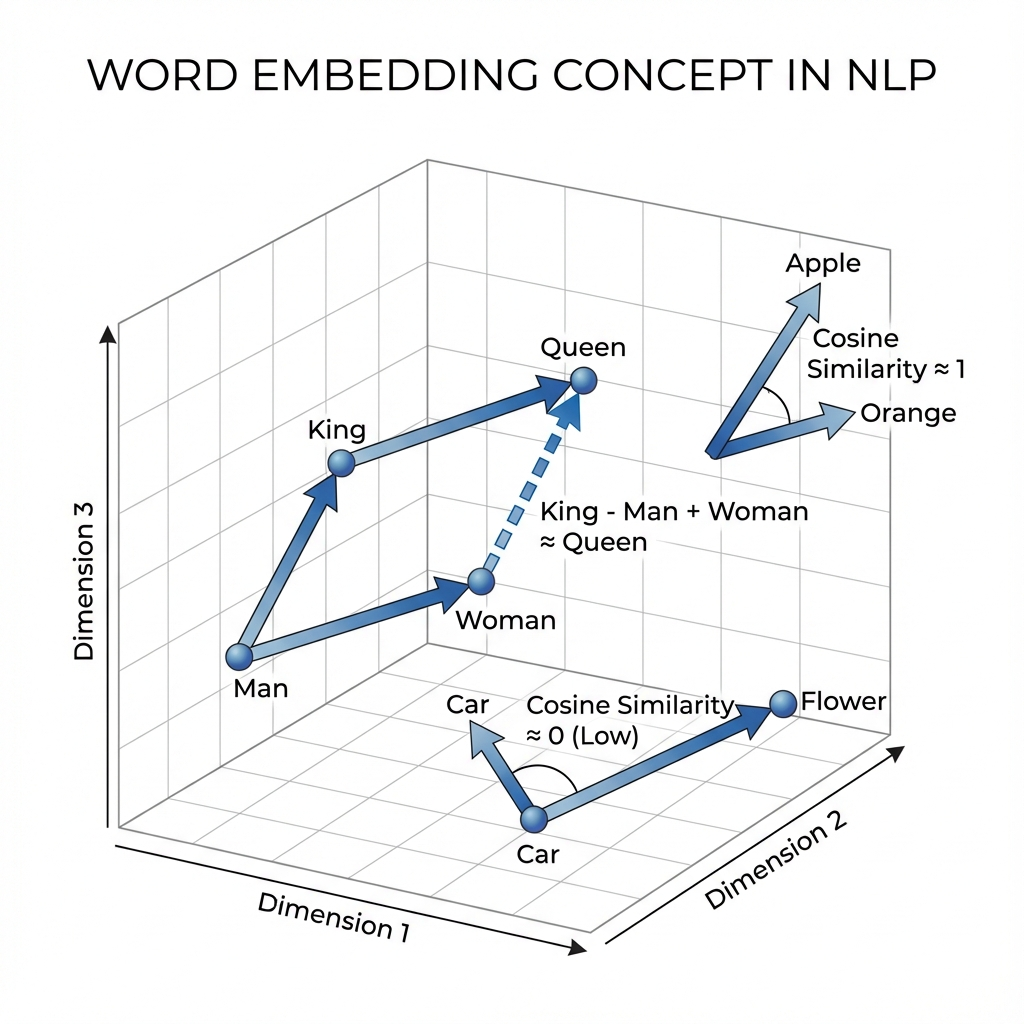
\includegraphics[width=0.7\textwidth]{Images/word_embedding.png}
    \caption{Minh họa không gian vector embedding và độ tương đồng cosine giữa các từ}
    \label{fig:word_embedding}
\end{figure}

Trong không gian embedding đa chiều (thường từ 512 đến 4096 chiều), các từ có ngữ nghĩa tương đồng sẽ có vector gần nhau. Độ tương đồng giữa hai vector thường được đo bằng cosine similarity:

\begin{equation}
\text{cosine\_similarity}(\mathbf{a}, \mathbf{b}) = \frac{\mathbf{a} \cdot \mathbf{b}}{\|\mathbf{a}\| \cdot \|\mathbf{b}\|} = \frac{\sum_{i=1}^{n} a_i b_i}{\sqrt{\sum_{i=1}^{n} a_i^2} \cdot \sqrt{\sum_{i=1}^{n} b_i^2}}
\end{equation}

Việc embedding giúp ``làm dày'' ngữ cảnh của mỗi data point, cho phép mô hình học được các mối quan hệ ngữ nghĩa phức tạp như:
\begin{itemize}
    \item $\text{vector}(\text{``King''}) - \text{vector}(\text{``Man''}) + \text{vector}(\text{``Woman''}) \approx \text{vector}(\text{``Queen''})$
    \item Các từ đồng nghĩa có vector gần nhau trong không gian embedding
    \item Các từ trong cùng ngữ cảnh có cosine similarity cao
\end{itemize}

\textbf{Cơ chế Self-Attention}

\begin{figure}[h!]
    \centering
    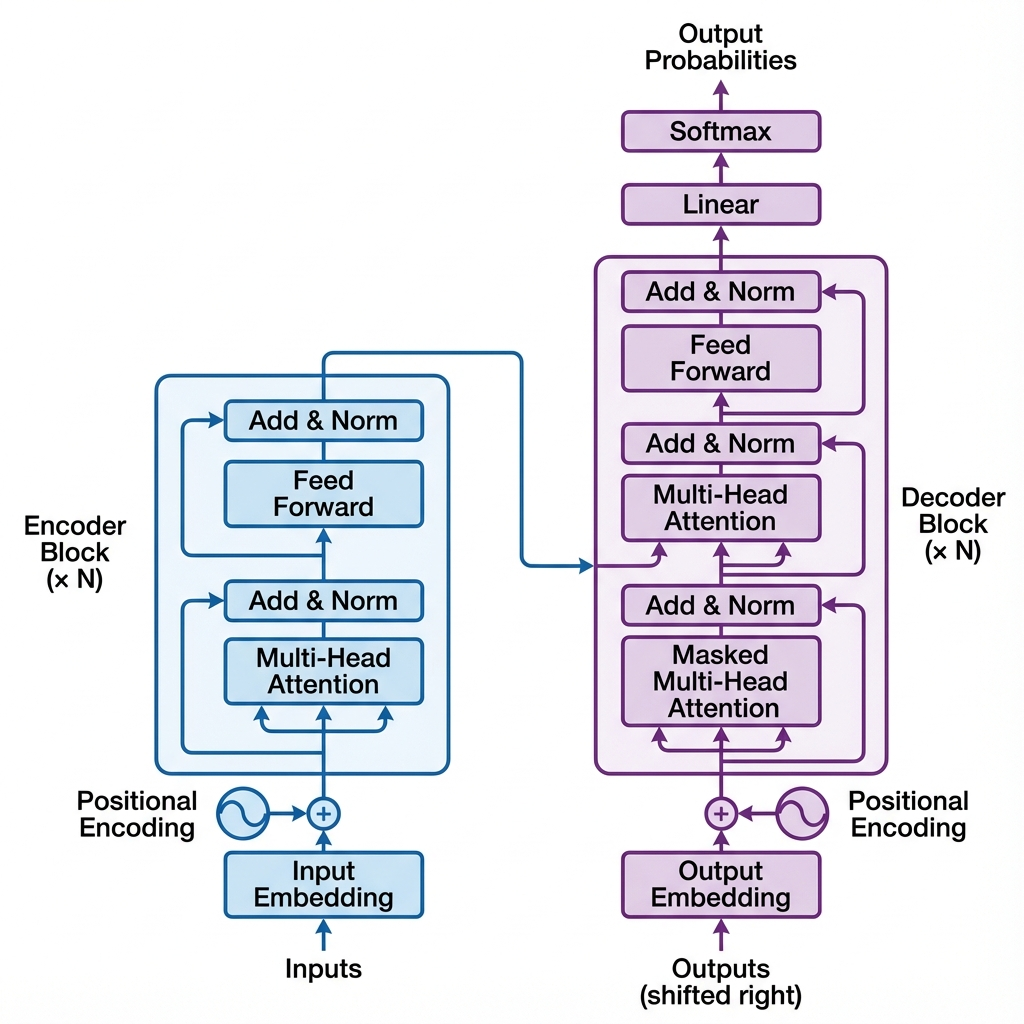
\includegraphics[width=0.8\textwidth]{Images/transformer_architecture.png}
    \vspace{6pt}
    \caption{Kiến trúc Transformer với các khối Encoder và Decoder}
    \label{fig:transformer_architecture}
\end{figure}
\begin{figure}[h!]
    \centering
    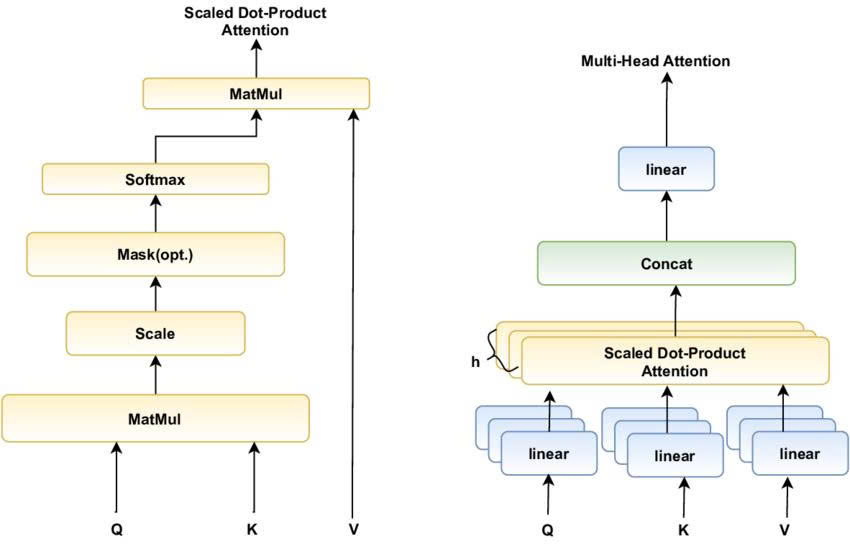
\includegraphics[width=0.85\textwidth]{Images/Self-Attention.jpg}
    \vspace{8pt}
    \caption{Cơ chế Self-Attention: Query, Key, Value và Scaled Dot-Product Attention}
    \label{fig:self_attention}
\end{figure}
Self-Attention cho phép mỗi vị trí trong chuỗi đầu vào ``chú ý'' đến tất cả các vị trí khác, học được mối quan hệ giữa các từ bất kể khoảng cách. Cơ chế này hoạt động thông qua ba ma trận: Query (Q), Key (K), và Value (V):

\begin{equation}
\text{Attention}(Q, K, V) = \text{softmax}\left(\frac{QK^T}{\sqrt{d_k}}\right)V
\end{equation}

Trong đó:
\begin{itemize}
    \item $Q$ (Query): Biểu diễn ``câu hỏi'' - token hiện tại muốn tìm thông tin gì
    \item $K$ (Key): Biểu diễn ``chìa khóa'' - các token khác chứa thông tin gì
    \item $V$ (Value): Biểu diễn ``giá trị'' - nội dung thực sự của các token
    \item $d_k$: Chiều của vector key, dùng để scale gradient ổn định
\end{itemize}

Multi-Head Attention mở rộng cơ chế này bằng cách chạy song song nhiều attention head, mỗi head học các loại quan hệ khác nhau:

\begin{equation}
\text{MultiHead}(Q, K, V) = \text{Concat}(\text{head}_1, ..., \text{head}_h)W^O
\end{equation}

Trong đó mỗi head được tính toán độc lập: $\text{head}_i = \text{Attention}(QW_i^Q, KW_i^K, VW_i^V)$

\textbf{Ưu điểm của Multi-Head Attention:}
\begin{itemize}
    \item \textbf{Đa dạng hóa biểu diễn}: Mỗi head có thể học các loại quan hệ khác nhau (ví dụ: head 1 học quan hệ cú pháp, head 2 học quan hệ ngữ nghĩa, head 3 học quan hệ vị trí).

    \item \textbf{Tối ưu hóa song song trên GPU}: Việc chia thành nhiều head độc lập cho phép tận dụng tối đa khả năng tính toán song song của GPU. Thay vì thực hiện một phép attention lớn với chiều $d_{model}$, ta thực hiện $h$ phép attention nhỏ với chiều $d_k = d_{model}/h$ song song. Điều này phù hợp hoàn hảo với kiến trúc SIMD (Single Instruction Multiple Data) của GPU, giúp:
    \begin{itemize}
        \item Tăng tốc độ training đáng kể nhờ batch matrix multiplication
        \item Tối ưu hóa throughput trong inference
        \item Sử dụng hiệu quả băng thông bộ nhớ GPU (memory bandwidth)
        \item Cho phép scale lên nhiều GPU dễ dàng hơn với tensor parallelism
    \end{itemize}

    \item \textbf{Giảm chi phí tính toán}: Tổng chi phí tính toán tương đương với single-head attention có cùng chiều $d_{model}$, nhưng hiệu quả hơn nhờ song song hóa.
\end{itemize}

\textbf{So sánh Transformer và CNN: Global Context vs Local Context}

Một trong những điểm mấu chốt của Transformer so với CNN là cách nắm bắt ngữ cảnh:

\begin{table}[h!]
\centering
\caption{So sánh Transformer và CNN}
\begin{tabular}{|l|p{6cm}|p{6cm}|}
\hline
\textbf{Đặc điểm} & \textbf{Transformer} & \textbf{CNN} \\
\hline
\textbf{Ngữ cảnh} & Global Context - Mỗi token có thể attention đến tất cả các token khác trong chuỗi & Local Context - Chỉ nhìn thấy các phần tử trong receptive field (kernel window) \\
\hline
\textbf{Inductive Bias} & Ít inductive bias $\rightarrow$ Cần lượng dữ liệu rất lớn để học & Có inductive bias mạnh về locality và translation equivariance \\
\hline
\textbf{Dữ liệu cần} & Yêu cầu dataset khổng lồ (hàng trăm GB văn bản) & Có thể hoạt động tốt với dataset nhỏ hơn \\
\hline
\textbf{Phức tạp} & $O(n^2)$ với độ dài chuỗi $n$ & $O(n \cdot k^2)$ với kernel size $k$ \\
\hline
\textbf{Ưu điểm} & Học được long-range dependencies tốt & Hiệu quả với dữ liệu có cấu trúc không gian (ảnh) \\
\hline
\end{tabular}
\end{table}

\textbf{Inductive Bias:} Transformer có rất ít giả định tiên nghiệm về cấu trúc dữ liệu (minimal inductive bias). Điều này có nghĩa là mô hình phải học toàn bộ ngữ cảnh và các pattern từ dữ liệu, thay vì có sẵn các ``bias'' như locality trong CNN. Hệ quả là Transformer cần lượng dữ liệu huấn luyện cực lớn để đạt được hiệu suất tốt.

\textbf{Kiến trúc Encoder-Decoder và Decoder-Only}

Transformer gốc bao gồm cả khối Encoder và Decoder:
\begin{itemize}
    \item \textbf{Encoder}: Xử lý chuỗi đầu vào, tạo biểu diễn ngữ cảnh. Sử dụng bidirectional attention (nhìn cả trái và phải).
    \item \textbf{Decoder}: Sinh chuỗi đầu ra từng token một, sử dụng cross-attention để tham chiếu đến encoder output.
\end{itemize}

Tuy nhiên, các mô hình sinh văn bản như GPT chỉ sử dụng \textbf{Decoder-Only} architecture với cơ chế \textbf{Masked Self-Attention} (hay Causal Attention):

\begin{equation}
\text{Masked-Attention}(Q, K, V) = \text{softmax}\left(\frac{QK^T}{\sqrt{d_k}} + M\right)V
\end{equation}

Trong đó $M$ là ma trận mask với $M_{ij} = -\infty$ nếu $j > i$ (các vị trí tương lai bị che). Điều này đảm bảo:
\begin{itemize}
    \item Mỗi token chỉ attend được đến các token trước nó (autoregressive)
    \item Tránh ``học vẹt'' (data leakage) - mô hình không thể nhìn thấy câu trả lời khi đang dự đoán
    \item Phù hợp cho các tác vụ sinh văn bản (text generation)
\end{itemize}

\textbf{Các Khối Phụ trợ trong Transformer}

\begin{itemize}
    \item \textbf{Layer Normalization}: Khác với Batch Normalization trong CNN, Layer Norm chuẩn hóa theo chiều feature thay vì theo batch. Điều này phù hợp hơn cho sequence data có độ dài thay đổi:
    \begin{equation}
    \text{LayerNorm}(x) = \gamma \cdot \frac{x - \mu}{\sqrt{\sigma^2 + \epsilon}} + \beta
    \end{equation}

    \item \textbf{Residual Connection}: Skip connection giúp gradient flow tốt hơn và cho phép đào tạo các mạng rất sâu.

    \item \textbf{Feed-Forward Network (FFN)}: Mỗi layer có một FFN với hidden dimension lớn (thường 4x embedding dimension):
    \begin{equation}
    \text{FFN}(x) = \max(0, xW_1 + b_1)W_2 + b_2
    \end{equation}

    \item \textbf{Positional Encoding}: Vì Transformer không có khái niệm về thứ tự, positional encoding được thêm vào để mã hóa vị trí của các token trong chuỗi.
\end{itemize}

\textbf{b) Các mô hình LLM tiêu biểu và các bước ngoặt}

Sự phát triển của LLM đã trải qua nhiều bước ngoặt quan trọng:

\textbf{Các bước ngoặt trong lịch sử LLM:}
\begin{enumerate}
    \item \textbf{GPT-1 (2018)}: OpenAI giới thiệu khái niệm pre-training + fine-tuning, chứng minh unsupervised pre-training có thể cải thiện NLP tasks.

    \item \textbf{BERT (2018)}: Google đề xuất bidirectional pre-training với masked language modeling, tạo bước đột phá trong NLU (Natural Language Understanding).

    \item \textbf{GPT-3 (2020)}: Với 175 tỷ tham số, GPT-3 chứng minh khả năng few-shot learning mà không cần fine-tuning, mở ra kỷ nguyên prompt engineering.

    \item \textbf{ChatGPT (2022)}: Sử dụng RLHF (Reinforcement Learning from Human Feedback) để align với mong muốn người dùng, tạo AI conversational thực sự hữu ích.

    \item \textbf{GPT-4 (2023)}: Mô hình đa phương thức (multimodal) có thể xử lý cả văn bản và hình ảnh, reasoning ability được cải thiện đáng kể.

    \item \textbf{Open-source revolution (2023-2024)}: LLaMA (Meta), Mistral, Qwen mở cửa cho cộng đồng nghiên cứu và triển khai local.

    \item \textbf{DeepSeek (2024)}: Bước ngoặt quan trọng từ Trung Quốc, DeepSeek-V3 đạt hiệu suất cạnh tranh với GPT-4 với chi phí huấn luyện thấp hơn đáng kể (chỉ \$5.6M), chứng minh hiệu quả của kiến trúc Mixture of Experts (MoE) và kỹ thuật Multi-head Latent Attention (MLA).
\end{enumerate}

\textbf{Bảng so sánh các mô hình LLM tiêu biểu:}

\begin{table}[h!]
\centering
\resizebox{\textwidth}{!}{
\begin{tabular}{|l|c|c|c|c|c|}
\hline
\textbf{Mô hình} & \textbf{Nhà phát triển} & \textbf{Tham số} & \textbf{Open-source} & \textbf{Đa phương thức} & \textbf{Đặc điểm nổi bật} \\
\hline
GPT-4o & OpenAI & N/A & Không & Có & SOTA reasoning, API phổ biến \\
\hline
Gemini 2.0 & Google & N/A & Không & Có & Tích hợp Google Search, dài context \\
\hline
Claude 3.5 & Anthropic & N/A & Không & Có & An toàn, coding mạnh \\
\hline
LLaMA 3.1 & Meta & 8B-405B & Có & Hạn chế & Cộng đồng lớn, dễ fine-tune \\
\hline
Mistral Large & Mistral AI & 7B-123B & Có & Có & Nhẹ, hiệu quả cho edge \\
\hline
Qwen 2.5 & Alibaba & 0.5B-72B & Có & Có & Đa ngôn ngữ, nhiều size \\
\hline
DeepSeek-V3 & DeepSeek & 671B MoE & Có & Có & Chi phí thấp, MoE hiệu quả \\
\hline
\end{tabular}
}
\label{tab:llm_comparison}
\end{table}

\textbf{Xu hướng hiện tại trong LLM:}
\begin{itemize}
    \item \textbf{Mixture of Experts (MoE)}: Chỉ kích hoạt một phần nhỏ tham số mỗi lần, giảm chi phí inference (DeepSeek, Mixtral).
    \item \textbf{Long context}: Mở rộng context window lên 128K-2M tokens (Gemini, Claude).
    \item \textbf{Multimodal}: Xử lý văn bản, hình ảnh, âm thanh, video trong cùng một mô hình.
    \item \textbf{Edge deployment}: Các mô hình nhỏ (1B-7B) chạy được trên smartphone và thiết bị nhúng.
    \item \textbf{Reasoning}: Cải thiện khả năng suy luận logic và toán học (o1, DeepSeek-R1).
\end{itemize}


\textbf{c) Kỹ thuật Prompt Engineering}

Prompt engineering là nghệ thuật thiết kế câu lệnh (prompt) để điều khiển hành vi của LLM. Các kỹ thuật prompting chính được so sánh trong bảng sau:

\begin{table}[h!]
\centering
\resizebox{\textwidth}{!}{
\begin{tabular}{|l|p{4cm}|p{5cm}|p{3cm}|}
\hline
\textbf{Kỹ thuật} & \textbf{Mô tả} & \textbf{Ví dụ prompt} & \textbf{Phù hợp với} \\
\hline
Zero-shot & Yêu cầu trực tiếp không có ví dụ & ``Dịch sang tiếng Anh: Xin chào'' & Tác vụ đơn giản \\
\hline
Few-shot & Cung cấp 2-5 ví dụ mẫu trước khi hỏi & ``Ví dụ: Mèo $\rightarrow$ Cat. Chó $\rightarrow$ Dog. Nhà $\rightarrow$ ?'' & Tác vụ cần định dạng cụ thể \\
\hline
System Prompt & Định nghĩa vai trò và quy tắc cho agent & ``Bạn là trợ lý y tế, luôn khuyên bệnh nhân gặp bác sĩ'' & Chatbot, AI Agent \\
\hline
\end{tabular}
}
\label{tab:prompting_techniques}
\end{table}

%=========================================

\subsubsection{Hệ thống chuyển đổi Giọng nói (STT \& TTS)}

Để tạo ra một vòng lặp giao tiếp tự nhiên hoàn chỉnh giữa người và máy (Human-Computer Interaction), hệ thống không chỉ xử lý văn bản mà còn phải nghe và nói. Điều này được thực hiện qua hai quy trình:

\begin{itemize}
    \item \textbf{Speech-to-Text (STT - Chuyển đổi Giọng nói thành Văn bản)}: Thu nhận sóng âm (audio waveform) từ microphone của robot, lọc nhiễu, phân tích phổ âm (spectrogram) và sử dụng các mô hình học sâu âm học để nhận diện và chuyển đổi thành chuỗi văn bản. Trong hệ thống này, văn bản thu được từ STT sẽ đóng vai trò làm câu lệnh (prompt) đầu vào cho LLM thông qua Groq API.
    \item \textbf{Text-to-Speech (TTS - Chuyển đổi Văn bản thành Giọng nói)}: Nhận chuỗi văn bản đầu ra từ LLM và tổng hợp thành tín hiệu âm thanh giọng nói con người. Hệ thống TTS hiện đại tạo ra giọng nói rất tự nhiên, có ngữ điệu và cảm xúc, giúp robot trở nên thân thiện hơn khi trò chuyện, nhắc nhở uống thuốc hoặc cảnh báo nguy hiểm.
\end{itemize}

Sự kết hợp giữa STT, Groq API (LLM siêu tốc) và TTS tạo nên một "bộ não" giao tiếp bằng giọng nói liên tục, đóng vai trò như một người bạn đồng hành ảo, hỗ trợ tương tác tự nhiên tối đa cho người cao tuổi vốn không quen thao tác trên màn hình cảm ứng.


% --- Tích hợp từ phần cũ ---
\subsubsection{Một số giải pháp Nhận dạng Giọng nói:}

Dưới đây là bảng so sánh các giải pháp chuyển đổi giọng nói thành văn bản (Speech-to-Text) phổ biến hiện nay:

\begin{table}[htbp]
\centering
\small
\begin{tabularx}{\textwidth}{@{} l >{\raggedright\arraybackslash}X >{\raggedright\arraybackslash}X >{\raggedright\arraybackslash}X @{}}
\toprule
\textbf{Tiêu chí} & \textbf{Google Speech-to-Text} & \textbf{OpenAI Whisper} & \textbf{Vosk} \\ \midrule
\textbf{Hình thức} & Cloud API (SaaS) & Open-source (Local/Cloud) & Open-source (Local) \\
\textbf{Độ chính xác} & Rất cao (đặc biệt tiếng Việt) & Cực cao (State-of-the-art) & Khá (tùy thuộc model) \\
\textbf{Internet} & Bắt buộc & Không bắt buộc & Không cần thiết \\
\textbf{Tốc độ} & Phụ thuộc băng thông & Phụ thuộc GPU/CPU & Rất nhanh (Real-time) \\
\textbf{Chi phí} & Trả phí theo lưu lượng & Miễn phí phần mềm & Miễn phí \\
\textbf{Phù hợp} & Ứng dụng mobile cần độ chính xác tối đa. & Robot có phần cứng mạnh, cần hiểu ngữ cảnh sâu. & Thiết bị nhúng (Raspberry Pi), phản hồi cực nhanh. \\ \bottomrule
\end{tabularx}
\caption{So sánh các công nghệ Speech-to-Text.}
\end{table}

\subsubsection{Phương pháp tiếp cận Xử lý Ngôn ngữ Tự nhiên (NLP) trong dự án}

Thay vì tự phát triển các mô hình NLP cục bộ (như Rule-based hay phân loại Intent bằng Machine Learning) vốn bị hạn chế về khả năng hiểu ngữ cảnh tự nhiên, hoặc triển khai trực tiếp các mô hình Deep Learning lớn gây quá tải cho phần cứng robot (edge devices), đồ án tiếp cận theo hướng hoàn toàn dựa vào API.

Cụ thể, hệ thống không huấn luyện hay lưu trữ mô hình ngôn ngữ riêng mà gọi trực tiếp \textbf{Groq API} để xử lý văn bản (sau khi âm thanh được STT dịch ra). Để duy trì tính mạch lạc trong giao tiếp (contextual memory), hệ thống không sử dụng các giải pháp lưu trữ phức tạp hay RAG, mà đơn giản sử dụng cơ chế \textbf{Session Chat} (Lưu trữ phiên trò chuyện). Trong cơ chế này, lịch sử của một vài vòng thoại gần nhất được lưu tạm thời trên RAM của ứng dụng và đính kèm vào phần \textit{prompt} gửi đi mỗi lần. Nhờ vậy, LLM có thể "nhớ" được ngữ cảnh trò chuyện ngắn hạn, giúp phản hồi tự nhiên hơn với chi phí lập trình và tài nguyên hệ thống thấp nhất.


\subsubsection{Phương thức triển khai: Điện toán Biên (Edge Computing) trên thiết bị Android}
Để đảm bảo hệ thống phản hồi theo thời gian thực, bảo vệ quyền riêng tư và tối ưu hóa băng thông mạng, đồ án đặt trọng tâm vào phương thức triển khai \textbf{Edge Computing} (Điện toán biên) trực tiếp trên thiết bị Android (Smartphone).

Toàn bộ các luồng xử lý cốt lõi bao gồm: thu nhận hình ảnh từ camera, chạy mô hình phát hiện đối tượng (YOLO26), theo dõi đa đối tượng (ByteTrack), và phân tích chuỗi thời gian bằng mạng LSTM để phát hiện té ngã, đều được thực thi hoàn toàn ở thiết bị biên thông qua bộ tăng tốc phần cứng (NPU/GPU trên điện thoại) kết hợp với các runtime như TensorFlow Lite.

Việc triển khai Edge Computing mang lại các ưu điểm vượt trội:
\begin{itemize}
    \item \textbf{Độ trễ thấp (Low Latency):} Xử lý ảnh tại chỗ giúp robot phát hiện người ngã ngay lập tức mà không phải chờ dữ liệu gửi lên và tải về từ server.
    \item \textbf{Đảm bảo quyền riêng tư (Privacy):} Dữ liệu hình ảnh sinh hoạt riêng tư của người cao tuổi không bị truyền ra ngoài môi trường Internet.
    \item \textbf{Độ tin cậy cao:} Hệ thống vẫn hoạt động ổn định các tính năng cốt lõi ngay cả khi mất kết nối mạng.
\end{itemize}
Riêng với tính năng giao tiếp hội thoại (NLP/Chat), thiết bị mới đóng vai trò làm client gọi Groq API (như đã trình bày) nhằm tận dụng năng lực suy luận ngôn ngữ, trong khi toàn bộ phần nhận thức thị giác máy tính và phân tích hành vi đều vận hành độc lập theo mô hình Edge Computing thuần túy.







\subsection{Giới thiệu Dataset Fall Detection – LE2I}
%=========================================

\subsubsection{Mục tiêu và đặc điểm của dataset LE2I}

LE2I Fall Detection Dataset là một trong những bộ dữ liệu chuẩn mực và phổ biến nhất dành cho bài toán phát hiện té ngã, được phát triển bởi phòng thí nghiệm Le2i (Đại học Burgundy, Pháp). Bộ dữ liệu cung cấp các video mô phỏng các hoạt động thường ngày (Activities of Daily Living - ADL) và các tình huống té ngã đa dạng \reportcite{ref:le2i}.

Đặc điểm nổi bật của dataset LE2I:
\begin{itemize}
    \item \textbf{Môi trường thực tế}: Được quay ở 4 bối cảnh khác nhau bao gồm: Nhà ở (Home), Phòng cafe (Coffee room), Văn phòng (Office) và Phòng học (Lecture room).
    \item \textbf{Đa dạng kịch bản ngã}: Bao gồm ngã về phía trước, phía sau, ngã do mất thăng bằng, hoặc ngã khi đang cố gắng đứng lên.
    \item \textbf{Nhiễu tự nhiên}: Video chứa các thách thức thực tế như đổ bóng (shadows), thay đổi ánh sáng (illumination variations), và che khuất (occlusions) do đồ vật.
\end{itemize}

\subsubsection{Dữ liệu video và Annotation}

Dataset LE2I bao gồm khoảng 191 video với các đặc điểm:
\begin{figure}[h!]
    \centering
    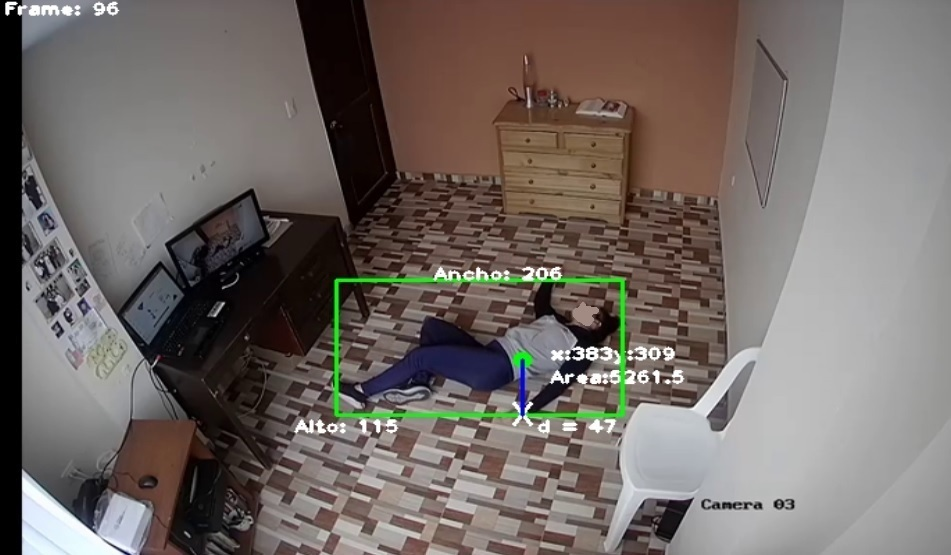
\includegraphics[width=0.85\textwidth]{Images/1.jpeg}
    \caption{Một số khung hình minh họa trong môi trường của dataset LE2I.}
\end{figure}
\begin{itemize}
    \item Độ phân giải video là 320x240 pixels với tốc độ khung hình 25 FPS.
    \item Annotation cung cấp khung hình bắt đầu và kết thúc quá trình ngã (ground truth frame numbers), kết hợp với thông tin Bounding Box của người.
    \item Các nhãn cơ bản gồm trạng thái ngã (fall) và hoạt động bình thường (no\_fall).
\end{itemize}

\subsubsection{Ưu điểm và hạn chế của dataset LE2I}

\textbf{Ưu điểm:}
\begin{itemize}
    \item Bối cảnh phong phú, từ không gian chật hẹp (văn phòng) đến rộng rãi (phòng học).
    \item Các tình huống ngã được diễn viên thực hiện tự nhiên, bao gồm các hoạt động khó phân biệt như cúi nhặt đồ hoặc ngồi xuống nhanh.
    \item Là chuẩn đối sánh (benchmark) uy tín được sử dụng rộng rãi trong các nghiên cứu Fall Detection.
\end{itemize}

\textbf{Hạn chế:}
\begin{itemize}
    \item Độ phân giải video tương đối thấp (320x240) so với các chuẩn camera HD hiện đại.
    \item Số lượng chủ thể (diễn viên) còn hạn chế so với các dataset quy mô lớn gần đây.
\end{itemize}

\subsubsection{So sánh với các Dataset quy mô lớn (DiverseFALL10500)}

Gần đây, một số nghiên cứu đề xuất các bộ dữ liệu khổng lồ như DiverseFALL10500 (10,500 ảnh) để khắc phục nhược điểm của các dataset cũ \reportcite{ref:falldetection}.

\textbf{So sánh LE2I và DiverseFALL10500:}
\begin{center}
\begin{tabular}{|l|c|c|}
\hline
\textbf{Tiêu chí} & \textbf{LE2I Dataset} & \textbf{DiverseFALL10500} \\
\hline
Số lượng video/ảnh & 191 videos & 10,500 images \\
Môi trường & 4 môi trường trong nhà & Indoor + Outdoor \\
Độ phân giải & 320x240 & Đa dạng (HD) \\
Yếu tố che khuất & Tích hợp sẵn (bàn, ghế) & Đa dạng \\
\hline
\end{tabular}
\end{center}

Đồ án này lựa chọn sử dụng (hoặc kết hợp) LE2I do đặc thù bộ dữ liệu này phản ánh rất sát các kịch bản trong môi trường nhà ở và có chứa chuỗi chuyển động thời gian (video), vô cùng phù hợp để trích xuất Tracklet cho mô hình LSTM.

%=========================================
\subsection{Suy luận AI trên thiết bị và TensorFlow Lite}

Edge AI xử lý dữ liệu gần nguồn thay vì gửi toàn bộ lên cloud. Với camera trong nhà, cách này giảm lưu lượng, độ trễ và phạm vi truyền ảnh; đồng thời vẫn cần kiểm soát quyền và lưu trữ cục bộ. TensorFlow Lite cung cấp runtime cho thiết bị di động/biên, hỗ trợ interpreter CPU và delegate phần cứng \reportcite{ref:tflite}.

Chuỗi chuyển đổi thường gồm model huấn luyện $\rightarrow$ biểu diễn trung gian $\rightarrow$ TFLite. Ba vấn đề phải kiểm chứng là: shape/layout tensor; toán tử được runtime/delegate hỗ trợ; và sai số số học sau tối ưu. FP16 giảm kích thước trọng số và băng thông bộ nhớ, nhưng không bảo đảm tăng tốc nếu delegate không sử dụng FP16. INT8 có thể giảm sâu hơn nhưng cần representative dataset và kiểm tra suy giảm keypoint/metric.

NMS có thể đặt trong graph hoặc ngoài graph. NMS trong graph giảm code hậu xử lý nhưng dễ tạo toán tử không tương thích delegate. NMS ngoài graph yêu cầu decoder Kotlin chính xác, đổi lại graph gọn và dễ chạy GPU hơn. Vì vậy kết quả chuyển đổi cần so ở cả tensor và detection cuối cùng.

\subsection{Firebase Authentication và Realtime Database}

Realtime Database tổ chức dữ liệu thành cây JSON và đồng bộ thay đổi tới client đang lắng nghe \reportcite{ref:firebase_rtdb}. Client Android có cache và hàng đợi write, do đó callback ``gần thời gian thực'' không đồng nghĩa bản ghi luôn mới. Đối với lệnh robot, timestamp/expiry là phần của ngữ nghĩa dữ liệu, không chỉ là metadata.

Firebase Authentication cung cấp UID cho người dùng; Security Rules chạy phía máy chủ quyết định read/write và có thể validate kiểu/cấu trúc \reportcite{ref:firebase_security}. Rules mặc định cần từ chối, sau đó cấp quyền tối thiểu theo UID, family và robot. Các node lệnh/signaling không nên dùng chung toàn cục trong hệ thống nhiều robot. Chúng cũng cần validate miền giá trị, người gửi và vòng đời phiên.

Ưu điểm của RTDB là tích hợp Android nhanh, listener đơn giản và phù hợp state/event nhỏ. Hạn chế là schema phi quan hệ, truy vấn có giới hạn và dễ tạo coupling bằng string path. Tách repository/data access, định nghĩa model chung và test rules bằng emulator giúp giảm rủi ro.

\subsection{WebRTC, signaling và ICE}

WebRTC là tập API/giao thức cho media và dữ liệu thời gian thực giữa các peer \reportcite{ref:webrtc}. Một phiên cần signaling để trao đổi Session Description Protocol (SDP) và ICE candidate, nhưng chuẩn không bắt buộc một công nghệ signaling cụ thể. Đề tài dùng RTDB cho phần này.

ICE thu thập candidate và kiểm tra cặp đường truyền để vượt Network Address Translator \reportcite{ref:ice}. STUN giúp peer biết địa chỉ public; TURN relay media khi không tạo được đường trực tiếp. Do đó có TURN làm tăng tỷ lệ kết nối nhưng thêm băng thông/độ trễ/chi phí máy chủ. Trạng thái call ở database và trạng thái PeerConnection là hai state machine khác nhau, cần cleanup idempotent để tránh phiên cũ.

WebRTC mã hóa media theo kiến trúc bảo mật giao thức, nhưng ứng dụng vẫn phải bảo vệ signaling, quyền camera/micro và danh tính peer \reportcite{ref:webrtc_security}. SDP/ICE có thể lộ thông tin mạng; log không nên lưu vô hạn. Trong hệ thống chăm sóc, phải có chỉ báo rõ khi camera/micro đang truyền.

\subsection{Bluetooth Low Energy và GATT}

BLE phù hợp liên kết cự ly gần giữa điện thoại và vi điều khiển. GATT xây trên bảng attribute, tổ chức dữ liệu thành service, characteristic và descriptor \reportcite{ref:ble_primer}. Server công bố service/characteristic; client quét, kết nối, khám phá và thực hiện read/write/notify theo property.

Write without response giảm round-trip và phù hợp dòng lệnh cập nhật thường xuyên, nhưng không có ACK ở tầng GATT cho từng write. Ứng dụng phải dùng gửi lặp, sequence/timestamp và watchdog. UUID 128-bit cho custom service tránh xung đột profile chuẩn. Payload văn bản dễ debug nhưng tốn byte và parser cần chặt; protocol nhị phân với version, sequence và checksum là hướng nâng cấp.

BLE disconnect là trạng thái bình thường có thể xảy ra do khoảng cách, radio hoặc vòng đời Android. Motor vì vậy không được giữ setpoint cuối. Callback disconnect và timeout độc lập ở firmware là yêu cầu an toàn, không nên chỉ dựa vào app.

\subsection{Động cơ BLDC và điều khiển FOC}

Động cơ BLDC/PMSM tạo mô-men bằng tương tác từ trường stator và rotor nam châm. Field-Oriented Control biến đổi dòng ba pha sang hệ trục quay $d$--$q$, tách thành phần từ thông và mô-men, sau đó dùng PWM để điều khiển điện áp \reportcite{ref:foc}. Với encoder từ AS5600, hệ thống có phản hồi góc/tốc độ cho vòng kín.

Vòng điều khiển vận tốc so sánh tốc độ đặt với tốc độ đo. PID có dạng khái quát:

\begin{equation}
u(t)=K_pe(t)+K_i\int_0^t e(\tau)d\tau+K_d\frac{de(t)}{dt}.
\end{equation}

Giới hạn điện áp bảo vệ driver/motor; giới hạn vận tốc bảo vệ cơ khí; lọc thông thấp giảm nhiễu đo. Deadzone giúp thắng ma sát tĩnh nhưng có thể tạo bước nhảy tốc độ, vì vậy bản hoàn thiện nên bổ sung ramp/giới hạn gia tốc. SimpleFOC cung cấp các abstraction motor, driver, sensor và vòng \texttt{loopFOC}/\texttt{move} cho vi điều khiển \reportcite{ref:simplefoc}.

\subsection{An toàn và quản trị rủi ro AI}

Một hệ thống cảnh báo người cao tuổi phải xem cả false positive và false negative. False positive lặp lại làm người dùng mất tin cậy; false negative có thể trì hoãn hỗ trợ. NIST AI RMF đề xuất các chức năng govern, map, measure và manage xuyên suốt vòng đời \reportcite{ref:nist_ai_rmf}. Với đồ án, điều này được cụ thể hóa bằng phạm vi sử dụng rõ, metric theo sự cố, log bằng chứng, giám sát lỗi, fallback và công bố giới hạn.

LLM không nên là thành phần duy nhất quyết định an toàn. Từ khóa cục bộ xử lý câu rõ, LLM chỉ phân loại trường hợp mơ hồ và lỗi mặc định nguy hiểm. Tương tự, output LSTM đi qua state machine/hậu kiểm. Các lớp độc lập làm hệ thống dễ kiểm tra hơn, nhưng không thay thế đánh giá thực địa.

\subsection{Kết luận chương}
%=========================================

Chương đã trình bày nền tảng robot dựa trên smartphone, mạng nơ-ron, CNN, detector họ YOLO, pose, dữ liệu té ngã, tracking, LSTM, LLM, nhận dạng giọng nói, AI biên, Firebase, WebRTC, BLE và FOC. Các nội dung được liên kết với lựa chọn hiện thực thay vì giả định một mô hình khảo sát chính là model cuối. Điểm then chốt là phát hiện té ngã của đề tài không dựa trên một nhãn ảnh duy nhất mà kết hợp pose, duy trì ID0, chuỗi LSTM và hậu kiểm có bằng chứng. Chương tiếp theo chuyển các khái niệm này thành yêu cầu, kiến trúc và hợp đồng cụ thể.
